% =====================================================================
%  Works with pdfLaTeX (default on Overleaf) and XeLaTeX/LuaLaTeX.
%  Upload the image files used below to the same Overleaf project
%  with the same file names (logo + figures).
% =====================================================================
\documentclass[12pt,a4paper]{article}

% ---------- page layout ----------
\usepackage[left=3cm,right=2cm,top=2cm,bottom=2cm]{geometry}
\setlength{\parindent}{0pt}
\setlength{\parskip}{6pt plus 2pt minus 1pt}
\linespread{1.1}
\setlength{\emergencystretch}{3em}

% ---------- fonts / Vietnamese ----------
\usepackage{iftex}
\ifPDFTeX
  \usepackage[T5]{fontenc}
  \usepackage[utf8]{inputenc}
  \usepackage{textcomp}
  \usepackage{tgtermes}            % Times-like font, supports Vietnamese
\else
  \usepackage{fontspec}
  % Use a Windows OpenType font when compiling with XeLaTeX/LuaLaTeX.
  % This avoids MiKTeX trying (and failing) to generate legacy metrics
  % for TeX Gyre Termes when that font package is not installed.
  \setmainfont{Times New Roman}
\fi
\usepackage{amsmath,amssymb}

% ---------- packages ----------
\usepackage{xcolor}
\usepackage{tikz}
\usepackage{graphicx}
\usepackage{adjustbox}
\usepackage{float}
\usepackage{needspace}
\usepackage{longtable,booktabs,array,calc}
\usepackage{etoolbox}
\usepackage{titlesec}
\usepackage[unicode,hidelinks]{hyperref}
\usepackage{bookmark}
\IfFileExists{xurl.sty}{\usepackage{xurl}}{}
\urlstyle{same}
\IfFileExists{microtype.sty}{\usepackage{microtype}}{}

\makeatletter
\patchcmd\longtable{\par}{\if@noskipsec\mbox{}\fi\par}{}{}
\makeatother

\providecommand{\tightlist}{\setlength{\itemsep}{0pt}\setlength{\parskip}{0pt}}
\newcolumntype{P}[1]{>{\raggedright\arraybackslash}p{#1}}

% no widows/orphans
\clubpenalty=10000 \widowpenalty=10000 \displaywidowpenalty=10000
% keep table captions together with their table (\np) / keep short tables whole (\npp)
\newcommand{\np}{\Needspace{8\baselineskip}}
\newcommand{\npp}{\Needspace{13\baselineskip}}
% bold label that must stay with the list below it
\newcommand{\lbl}[1]{\Needspace{6\baselineskip}\textbf{#1}\par\nopagebreak}
% minus sign usable in text
\newcommand{\mn}{\ensuremath{-}}

% ---------- headings ----------
\setcounter{secnumdepth}{-\maxdimen}   % titles are numbered by hand
\setcounter{tocdepth}{3}
\titleformat{\section}{\centering\bfseries\large}{}{0pt}{}
\titlespacing*{\section}{0pt}{0pt}{14pt}
\titleformat{\subsection}{\bfseries\normalsize}{}{0pt}{}
\titlespacing*{\subsection}{0pt}{14pt}{6pt}
\titleformat{\subsubsection}{\bfseries\itshape\normalsize}{}{0pt}{}
\titlespacing*{\subsubsection}{0pt}{10pt}{4pt}
% subsection headings never stranded at the bottom of a page
\let\oldsubsection\subsection
\renewcommand{\subsection}{\Needspace{12\baselineskip}\oldsubsection}
\let\oldsubsubsection\subsubsection
\renewcommand{\subsubsection}{\Needspace{10\baselineskip}\oldsubsubsection}
% every main part starts on a new page
\newcommand{\chap}[1]{\clearpage\section{#1}}

\renewcommand{\contentsname}{MỤC LỤC}
\definecolor{cmcblue}{HTML}{4A90E2}
\author{}
\date{}

\begin{document}

% =====================================================================
%  COVER PAGE
% =====================================================================
\newgeometry{margin=2.5cm}
\newcommand{\logowidth}{12cm}    % logo size
\newcommand{\logogap}{1.2cm}    % space between logo and the title
\begin{titlepage}
\thispagestyle{empty}
\begin{tikzpicture}[remember picture,overlay]
  \draw[cmcblue,line width=1.5pt]
    ([xshift=1.2cm,yshift=-1.2cm]current page.north west) rectangle
    ([xshift=-1.2cm,yshift=1.2cm]current page.south east);
\end{tikzpicture}
\centering
\vspace*{0.5cm}

{\large\bfseries TRƯỜNG ĐẠI HỌC CMC}\\[0.5cm]
{\large\bfseries Khoa Công nghệ thông tin \& Truyền thông}

\vspace{\stretch{1}}
\makebox[\textwidth][c]{\hspace*{4mm}
\includegraphics[width=\logowidth]{./Logo-Dai-hoc-CMC-V.png}}

\vspace{\logogap}

{\large\bfseries BÁO CÁO BÀI TẬP LỚN}\\[0.5cm]
{\large\bfseries HỌC PHẦN: TRÍ TUỆ NHÂN TẠO}\\[0.4cm]
{\normalsize\bfseries ĐỀ TÀI: Xây dựng mô hình tìm kiếm phim dựa trên từ khóa}\\[0.4cm]
{\normalsize\bfseries Ngành: Khoa học máy tính - Trí tuệ nhân tạo}\\[0.6cm]

{\large\bfseries Thành viên thực hiện:}\\[0.3cm]
\begingroup\small\bfseries
\begin{tabular}{@{}p{5.4cm}p{4.2cm}l@{}}
1. Nguyễn Trần Như Thành & Mã SV: BAI250059 & Lớp: 25AI \\[3pt]
2. Nguyễn Hiền Tiến       & Mã SV: BCS250036 & Lớp: 25CS \\[3pt]
3. Nguyễn Việt Trung      & Mã SV: BAI250064 & Lớp: 25AI \\[3pt]
4. Đinh Quang Tùng        & Mã SV: BAI250070 & Lớp: 25AI \\[3pt]
5. Trương Hoàng Việt      & Mã SV: BCS250040 & Lớp: 25CS \\
\end{tabular}
\endgroup

\vspace{\stretch{2}}
{\footnotesize\bfseries Giảng viên hướng dẫn: ThS. Vũ Việt Vũ}

\vspace*{0.5cm}
\end{titlepage}
\restoregeometry

% =====================================================================
%  TABLE OF CONTENTS + ABBREVIATIONS (roman page numbers)
% =====================================================================
\pagenumbering{roman}
\setcounter{page}{1}

{\setlength{\parskip}{0pt}\tableofcontents}

\clearpage
\section*{DANH MỤC TỪ VIẾT TẮT}
\addcontentsline{toc}{section}{DANH MỤC TỪ VIẾT TẮT}

{\def\LTcaptype{}\small
\begin{longtable}[]{@{}P{(\linewidth - 6\tabcolsep) * \real{0.0749}}P{(\linewidth - 6\tabcolsep) * \real{0.1281}}P{(\linewidth - 6\tabcolsep) * \real{0.4126}}P{(\linewidth - 6\tabcolsep) * \real{0.3844}}@{}}
\toprule
\textbf{STT} & \textbf{Từ viết tắt} & \textbf{Tiếng Anh} & \textbf{Nghĩa tiếng Việt} \\
\midrule
\endhead
\bottomrule
\endlastfoot
1 & ANN & Approximate Nearest Neighbor & Tìm láng giềng gần nhất xấp xỉ \\
2 & API & Application Programming Interface & Giao diện lập trình ứng dụng \\
3 & BERT & Bidirectional Encoder Representations from Transformers & Mô hình mã hóa hai chiều dựa trên Transformer \\
4 & BM25 & Okapi Best Matching 25 & Hàm xếp hạng văn bản theo tần suất từ \\
5 & CPU & Central Processing Unit & Bộ xử lý trung tâm \\
6 & FAISS & Facebook AI Similarity Search & Thư viện tìm kiếm vector \\
7 & fp16, fp32 & 16-bit, 32-bit floating point & Số thực dấu phẩy động 16 bit, 32 bit \\
8 & FTS5 & Full-Text Search 5 & Mô-đun tìm kiếm toàn văn của SQLite \\
9 & GPU & Graphics Processing Unit & Bộ xử lý đồ họa \\
10 & hit@k & Hit rate at k & Tỉ lệ truy vấn có phim đúng trong k kết quả đầu \\
11 & HNSW & Hierarchical Navigable Small World & Chỉ mục đồ thị phân tầng cho tìm láng giềng gần nhất xấp xỉ \\
12 & IDF & Inverse Document Frequency & Tần suất nghịch đảo văn bản \\
13 & IMDb & Internet Movie Database & Cơ sở dữ liệu phim IMDb \\
14 & LLM & Large Language Model & Mô hình ngôn ngữ lớn \\
15 & P@k & Precision at k & Độ chính xác trong k kết quả đầu \\
16 & p95 & 95th percentile & Phân vị thứ 95 \\
17 & R@k & Recall at k & Độ phủ trong k kết quả đầu \\
18 & RAM & Random Access Memory & Bộ nhớ truy cập ngẫu nhiên \\
19 & RRF & Reciprocal Rank Fusion & Ghép thứ hạng theo nghịch đảo hạng \\
20 & STT & --- & Số thứ tự \\
21 & TMDB & The Movie Database & Cơ sở dữ liệu phim TMDB \\
\end{longtable}
}

% =====================================================================
%  MỞ ĐẦU
% =====================================================================
\clearpage
\pagenumbering{arabic}
\setcounter{page}{1}
\section{MỞ ĐẦU}

Mô hình tinh chỉnh của nhóm đưa độ chính xác trong 10 kết quả đầu (P@10) từ 19,7\% lên 38,3\% so với mô hình gốc, và từ 17,5\% lên 30,8\% với các từ khóa chưa từng xuất hiện khi huấn luyện.

\textbf{Bối cảnh.} Người xem thường tìm phim theo nội dung họ nhớ hoặc muốn xem (``time travel'', ``heist'', ``twist ending''), không theo tên phim. Các trang phim phổ biến tìm theo tên, hoặc lọc theo thể loại, năm và diễn viên.

\textbf{Vấn đề.} Có hai cách truyền thống, cả hai đều yếu với loại truy vấn này:

\begin{itemize}
\tightlist
\item Tìm theo từ (BM25) chỉ trả về phim có đúng từ đó trong mô tả. Phim về du hành thời gian mà tóm tắt không ghi ``time travel'' sẽ bị bỏ sót.
\item Mô hình nhúng câu có sẵn (all-MiniLM-L6-v2) hiểu nghĩa tốt hơn nhưng vẫn bám vào bề mặt chữ: ``twist ending'' trả về \emph{Oliver Twist}, ``feel-good'' trả về \emph{I Feel Pretty}.
\end{itemize}

\textbf{Đối tượng.} Người xem phim dùng trang tìm kiếm; các trang cơ sở dữ liệu phim hoặc dịch vụ xem phim cần ô tìm kiếm theo nội dung.

\textbf{Lợi ích kỳ vọng.} Tinh chỉnh mô hình trên các cặp (từ khóa, phim) có sẵn từ cộng đồng MovieLens và TMDB, để mô hình học ý nghĩa của từ khóa theo cách người xem dùng. Không cần gán nhãn thủ công. Mô hình nhỏ (90,9 MB) nên chạy được trên CPU.

% =====================================================================
%  PHẦN I
% =====================================================================
\chap{PHẦN I. TỔNG QUAN}

\subsection{1.1. Giới thiệu bài toán}

Xây dựng hệ thống tìm kiếm phim: người dùng nhập một từ khóa hoặc câu mô tả (tiếng Anh), hệ thống trả về 20 phim phù hợp nhất trong danh mục 17.238 phim. Nhóm tinh chỉnh mô hình nhúng câu all-MiniLM-L6-v2 cho việc này và so sánh với BM25 và mô hình gốc.

\lbl{Dữ liệu}

\begin{itemize}
\tightlist
\item Danh mục phim từ IMDb: tên, năm, thể loại, điểm. Gồm phim có từ 10.000 lượt đánh giá trở lên (từ 2.000 với phim từ năm 2020), bỏ phim người lớn.
\item Tóm tắt nội dung và từ khóa từ TMDB.
\item Tag genome (1.128 thẻ, mỗi phim một điểm liên quan 0--1 cho từng thẻ) và thẻ do người dùng gắn từ MovieLens 25M.
\end{itemize}

Chi tiết ở Phần III.1.

\lbl{Các yêu cầu của hệ thống}

\begin{itemize}
\tightlist
\item Mục tiêu mô hình: xếp hạng (truy hồi thông tin). Với một truy vấn, sắp xếp phim theo mức phù hợp.
\item Phạm vi: phim trong danh mục, truy vấn tiếng Anh ngắn (từ khóa, cụm từ), tối đa 200 ký tự. Không xử lý truy vấn tiếng Việt, không cá nhân hóa theo người dùng.
\item Ràng buộc: huấn luyện trên GPU miễn phí của Google Colab (T4); suy luận trên CPU; không tốn phí API.
\item Nghiên cứu giải pháp: BM25, MiniLM gốc, MiniLM tinh chỉnh bằng học tương phản (Phần II), và ghép MiniLM tinh chỉnh với BM25 (Phần III.2.6).
\end{itemize}

\np\textbf{Bảng 1.1. Yêu cầu phi chức năng} (giá trị đo được ở Phần III.2.4)

{\def\LTcaptype{}\small
\begin{longtable}[]{@{}*{2}{P{(\linewidth - 2\tabcolsep) * \real{0.4947}}}@{}}
\toprule
\textbf{Yêu cầu} & \textbf{Tiêu chí} \\
\midrule
\endhead
\bottomrule
\endlastfoot
Độ chính xác & P@10 và R@100 cao hơn BM25 và mô hình gốc, kể cả với từ khóa không có trong tập huấn luyện \\
Độ trễ & Một truy vấn trả kết quả dưới 1 giây trên CPU \\
Bộ nhớ & Mô hình và vector của cả danh mục nằm trong RAM của một máy cá nhân \\
Khả năng mở rộng & Thêm phim mới chỉ cần nhúng văn bản của phim đó, không huấn luyện lại \\
Khả năng giải thích & Mỗi kết quả có điểm tương đồng cosine; người dùng xem được tóm tắt phim để tự kiểm tra \\
Độ tin cậy & Kết quả tái lập được: seed cố định, phiên bản thư viện cố định, kiểm tra rò rỉ dữ liệu bằng assert \\
\end{longtable}
}

\textbf{Báo cáo:} phương pháp (Phần II), thực nghiệm và đánh giá (Phần III), kết luận (Phần IV), hướng dẫn chạy và ảnh trang demo (Phụ lục).

\subsection{1.2. Một số thông tin liên quan}

\np\textbf{Bảng 1.2. Phân công nhiệm vụ}

{\def\LTcaptype{}\small
\begin{longtable}[]{@{}*{4}{P{(\linewidth - 6\tabcolsep) * \real{0.2361}}}@{}}
\toprule
\textbf{STT} & \textbf{Họ tên} & \textbf{Nội dung công việc} & \textbf{Nhận xét về tiến độ và chất lượng của Trưởng nhóm} \\
\midrule
\endhead
\bottomrule
\endlastfoot
1 & Trương Hoàng Việt & Xây dựng cơ sở dữ liệu phim: IMDb, TMDB, MovieLens & Hoàn thành đúng tiến độ, dữ liệu được làm sạch và đối chiếu chính xác giữa các nguồn. \\
2 & Đinh Quang Tùng & Chuẩn bị dữ liệu, thử nghiệm tối ưu mô hình & Đảm bảo tiến độ đề ra; kiểm tra phân chia dữ liệu, so sánh các phương án với baseline và ghi nhận kết quả thực nghiệm ở Phần III.3. \\
3 & Nguyễn Việt Trung & Tạo Notebook tinh chỉnh & Hoàn thành tốt và đúng hạn, mã nguồn huấn luyện chạy ổn định, dễ tái lập kết quả. \\
4 & Nguyễn Trần Như Thành & Đánh giá mô hình & Hoàn thành đúng tiến độ, phân tích kết quả chi tiết và đưa ra được các hướng cải tiến hiệu quả. \\
5 & Nguyễn Hiền Tiến & Review + duyệt báo cáo & Hoàn thành xuất sắc, kiểm tra kỹ lưỡng nội dung, đảm bảo tính logic, chính xác và đúng thời hạn trước khi nộp. \\
\end{longtable}
}

\subsection{1.3. Đạo đức và pháp lý}

\np\textbf{Bảng 1.3. Rủi ro đạo đức, pháp lý và biện pháp}

{\def\LTcaptype{}\small
\begin{longtable}[]{@{}*{3}{P{(\linewidth - 4\tabcolsep) * \real{0.3223}}}@{}}
\toprule
\textbf{Rủi ro} & \textbf{Hiện trạng} & \textbf{Biện pháp} \\
\midrule
\endhead
\bottomrule
\endlastfoot
Giấy phép dữ liệu & IMDb: chỉ dùng cá nhân, phi thương mại. MovieLens 25M: chỉ dùng cho nghiên cứu, cấm phân phối lại, phải trích dẫn. Bản TMDB trên Kaggle: Apache 2.0; dữ liệu gốc từ TMDB API & Không đưa dữ liệu thô lên git; mỗi thành viên tự tải về và xây dựng lại bằng script. Trích dẫn MovieLens; ghi nguồn TMDB trên sản phẩm. Chỉ dùng cho mục đích học tập. \\
Thiên lệch danh mục & Chỉ gồm phim nhiều lượt đánh giá trên IMDb, chủ yếu phim tiếng Anh; phim ít người biết không được tìm thấy & Nêu rõ phạm vi; hạ ngưỡng lượt đánh giá cho phim từ 2020 xuống 2.000 \\
Thiên lệch nhãn & Thẻ MovieLens do một nhóm người dùng (chủ yếu phương Tây) gắn; tag genome chỉ có cho phim đến 2019, nên tập kiểm thử không có phim mới & Thêm từ khóa TMDB (có cho cả phim mới) vào dữ liệu huấn luyện; ghi rõ giới hạn của tập kiểm thử \\
Quyền riêng tư & userId của MovieLens (đã ẩn danh) chỉ dùng để đếm số người gắn cùng một thẻ, không đi vào mô hình. Server không lưu truy vấn; uvicorn chỉ in dòng truy cập ra console & Không ghi log truy vấn ra file; không thu thập tài khoản người dùng \\
Nội dung nhạy cảm & Một số từ khóa TMDB mô tả bạo lực, tình dục; truy vấn kiểu này vẫn trả về phim tương ứng & Danh mục đã bỏ phim người lớn (cờ isAdult của IMDb) \\
Minh bạch & Trang demo không hiển thị điểm tương đồng; người dùng không biết vì sao một phim được xếp hạng & Báo cáo nêu rõ cách xếp hạng và độ chính xác đo được. Hướng phát triển: hiển thị điểm và từ khóa khớp \\
\end{longtable}
}

\subsection{1.4. Kết luận}

Bài toán là xếp hạng phim theo truy vấn ngắn. Dữ liệu huấn luyện lấy từ nhãn có sẵn của MovieLens và TMDB, không cần gán nhãn thủ công. Rủi ro chính là giấy phép dữ liệu và thiên lệch về phim phổ biến, phim cũ.

% =====================================================================
%  PHẦN II
% =====================================================================
\chap{PHẦN II. PHƯƠNG PHÁP THỰC HIỆN}

\subsection{1. Đặt vấn đề}

Mỗi phim $d$ được biểu diễn bằng một đoạn văn bản: Tên (Năm). Thể loại. Tóm tắt. Ví dụ: \emph{Rocky Balboa (2006). Drama, Sport. When he loses a highly publicized virtual boxing match\ldots{}} Với truy vấn $q$, mô hình tính điểm $s(q,d)$ cho mọi phim và trả về $k$ phim điểm cao nhất:

\[
\mathrm{top}_k(q) = \operatorname*{arg\,top\text{-}k}_{d \in D}\; s(q,d)
\]

Phim $d$ phù hợp với thẻ $t$ khi điểm tag genome $g(d,t) \geq 0{,}8$. Điểm này dùng làm đáp án khi đánh giá, nên thẻ không được đưa vào văn bản của phim.

\subsection{2. Một số mô hình giải quyết bài toán}

\subsubsection{2.1. BM25 (tìm theo từ)}

BM25 chấm điểm theo số lần từ của truy vấn xuất hiện trong văn bản, giảm trọng số cho từ phổ biến và văn bản dài:

\[
\mathrm{BM25}(q,d)=\sum_{w\in q}\mathrm{IDF}(w)\cdot
\frac{f(w,d)\,(k_1+1)}{f(w,d)+k_1\left(1-b+b\,\dfrac{|d|}{\mathrm{avgdl}}\right)}
\]

$f(w,d)$ là số lần từ $w$ xuất hiện trong $d$, $|d|$ là độ dài văn bản, avgdl là độ dài trung bình. Nhóm dùng bảng FTS5 của SQLite với bộ tách từ Porter (đưa từ về gốc: ``zombies'' $\rightarrow$ ``zombi'') và tham số mặc định $k_1 = 1{,}2$, $b = 0{,}75$. Các từ của truy vấn nối bằng OR. BM25 không cần huấn luyện nhưng không tìm được phim mô tả cùng ý bằng từ khác.

\subsubsection{2.2. MiniLM gốc (all-MiniLM-L6-v2)}

all-MiniLM-L6-v2 là mô hình Transformer 6 lớp (kiến trúc BERT, khoảng 22,7 triệu tham số), chưng cất từ MiniLM và huấn luyện sẵn bởi Sentence-Transformers trên hơn 1 tỷ cặp câu. Mô hình là bi-encoder: truy vấn và phim được mã hóa riêng thành vector 384 chiều. Vector lấy bằng trung bình các token (mean pooling) rồi chuẩn hóa về độ dài 1, nên điểm là cosine:

\[
s(q,d)=\cos\big(E(q),E(d)\big)=E(q)^{\top}E(d),\qquad \lVert E(\cdot)\rVert=1
\]

Vì phim được mã hóa riêng, vector của cả danh mục tính một lần khi khởi động. Mỗi truy vấn chỉ cần mã hóa một câu và nhân ma trận. Mô hình gốc học trên câu tổng quát, không phải trên cặp (từ khóa, phim), nên hay khớp theo chữ bề mặt.

\subsubsection{2.3. MiniLM tinh chỉnh bằng Multiple Negatives Ranking Loss}

Giữ nguyên kiến trúc và huấn luyện tiếp mô hình gốc trên các cặp $(a,p)$: $a$ là một thẻ hoặc từ khóa, $p$ là văn bản của một phim hợp với thẻ đó. Trong một lô $B$ cặp, phim của các cặp khác đóng vai mẫu âm (in-batch negatives). Hàm mất mát là cross-entropy trên điểm cosine nhân hệ số $\sigma = 20$:

\[
\mathcal{L}=-\frac{1}{B}\sum_{i=1}^{B}\log
\frac{\exp\big(\sigma\cos(a_i,p_i)\big)}{\sum_{j=1}^{B}\exp\big(\sigma\cos(a_i,p_j)\big)}
\]

Mô hình học kéo vector của thẻ lại gần phim hợp với nó và đẩy xa $B-1$ phim còn lại. Bộ lấy mẫu no\_duplicates không cho một thẻ hoặc một phim xuất hiện hai lần trong cùng lô, vì khi đó một cặp đúng sẽ bị tính là mẫu âm. Hạn chế: một phim khác trong lô vẫn có thể hợp với thẻ (ví dụ hai phim zombie) nhưng bị tính là mẫu âm.

\subsection{3. Kết luận}

\np\textbf{Bảng 2.1. So sánh các mô hình}

{\def\LTcaptype{}\small
\begin{longtable}[]{@{}*{4}{P{(\linewidth - 6\tabcolsep) * \real{0.2361}}}@{}}
\toprule
\textbf{Mô hình} & \textbf{Cần huấn luyện} & \textbf{Hiểu từ đồng nghĩa} & \textbf{Vai trò} \\
\midrule
\endhead
\bottomrule
\endlastfoot
BM25 & Không & Không & Mốc so sánh \\
MiniLM gốc & Không (dùng sẵn) & Có, theo nghĩa tổng quát & Mốc so sánh \\
MiniLM tinh chỉnh & Có, trên 236.365 cặp & Có, theo cách người xem gắn thẻ & Mô hình đề xuất \\
MiniLM tinh chỉnh lần 2 + BM25 (Phần III.2.6) & Có, trên 251.635 cặp & Có, cộng thêm khớp từ chính xác & Mô hình trên trang demo \\
\end{longtable}
}

Nhóm chọn MiniLM tinh chỉnh vì giữ được chi phí suy luận của mô hình gốc và học được nghĩa của từ khóa phim từ dữ liệu có sẵn.

% =====================================================================
%  PHẦN III
% =====================================================================
\chap{PHẦN III. THỰC NGHIỆM VÀ ĐÁNH GIÁ KẾT QUẢ}

Trên 1.798 phim kiểm thử chưa dùng khi huấn luyện, mô hình tinh chỉnh đạt P@10 = 38,3\% với thẻ đã thấy và 30,8\% với thẻ chưa thấy, so với 19,7\% và 17,5\% của mô hình gốc. Đổi lại, mô hình tìm theo tên phim kém hơn. Lần huấn luyện thứ hai thêm cặp (tên phim, văn bản phim), giữ nguyên P@10 và nâng tỉ lệ tên phim đứng đầu kết quả từ 27,0\% lên 62,5\% (Phần III.2.5). Ghép mô hình lần 2 với BM25 theo trọng số 80/20 giữ nguyên P@10 và tăng tỉ lệ này thêm 12,1 điểm (Phần III.2.6). Trang demo dùng cách ghép này.

\subsection{1. Dữ liệu thực nghiệm}

\subsubsection{1.1. Nguồn dữ liệu}

\np\textbf{Bảng 3.1. Nguồn dữ liệu}

{\def\LTcaptype{}\small
\begin{longtable}[]{@{}*{4}{P{(\linewidth - 6\tabcolsep) * \real{0.2361}}}@{}}
\toprule
\textbf{Nguồn} & \textbf{Dùng cho} & \textbf{Kích thước sau xử lý} & \textbf{Giấy phép} \\
\midrule
\endhead
\bottomrule
\endlastfoot
\href{https://datasets.imdbws.com/}{IMDb datasets} (title.basics, title.ratings) & Tên, năm, thể loại, điểm, số lượt đánh giá & 17.238 phim, 1915--2026, 23 thể loại & Cá nhân, phi thương mại \\
Bản TMDB trên Kaggle (TMDB\_\allowbreak all\_\allowbreak movies.csv, 806 MB) + TMDB API & Tóm tắt, từ khóa; ảnh poster cho demo & Tóm tắt: 17.100 phim. Từ khóa: 15.111 phim, 22.777 từ khóa khác nhau & Apache 2.0 (bản Kaggle); TMDB API yêu cầu ghi nguồn \\
\href{https://grouplens.org/datasets/movielens/25m/}{MovieLens 25M} tag genome & Điểm liên quan của 1.128 thẻ cho mỗi phim: nhãn huấn luyện và đáp án kiểm thử & 8.993 phim trong danh mục & Nghiên cứu, cấm phân phối lại \\
MovieLens 25M tags.csv, links.csv & Thẻ người dùng tự gõ; ánh xạ sang mã IMDb & 1.093.360 thẻ từ 14.592 người dùng cho 45.251 phim (trước khi lọc) & Nghiên cứu, cấm phân phối lại \\
\end{longtable}
}

\subsubsection{1.2. Quy trình thu thập, gán nhãn và làm sạch}

\begin{enumerate}
\def\labelenumi{\arabic{enumi}.}
\item \textbf{Lọc danh mục} (python -m moviebot.build\_db): phim lẻ và phim truyền hình trên IMDb, isAdult = 0, có năm phát hành, từ 10.000 lượt đánh giá (từ 2.000 với phim từ 2020). Kết quả: 17.238 phim.
\item \textbf{Ghép TMDB} (python -m moviebot.import\_tmdb): theo mã IMDb, điền tóm tắt và cột keywords (phân tách bằng \textbar). Không gọi API.
\item \textbf{Văn bản phim}: Tên (Năm). Thể loại. Tóm tắt. Bỏ 138 phim không có tóm tắt, còn 17.100 phim. Thẻ và từ khóa không đưa vào văn bản vì chúng là đáp án.
\item \textbf{Gán nhãn}: không gán thủ công. Cặp (thẻ, phim) lấy từ ba nguồn có sẵn:
  \begin{enumerate}
  \def\labelenumii{\alph{enumii}.}
  \item Tag genome: mọi thẻ có điểm $\geq 0{,}8$ với phim. 66.618 cặp.
  \item Thẻ người dùng: chuyển chữ thường, bỏ khoảng trắng thừa, dài tối đa 40 ký tự (thẻ dài hơn thường là cả câu), và ít nhất 2 người khác nhau gắn cùng thẻ cho cùng phim (bỏ nhãn cá nhân kiểu ``bd-r''). 69.273 cặp.
  \item Từ khóa TMDB: mỗi từ khóa của phim. 132.050 cặp.
  \item Gộp và bỏ trùng: 236.365 cặp.
  \end{enumerate}
\item \textbf{Chuẩn hóa thẻ khi chia tập}: hàm tag\_key chuyển chữ thường, bỏ ký tự không phải chữ số, bỏ s cuối, nên ``Zombie'' và ``zombies'' cùng một khóa. 1.128 thẻ genome thành 1.095 khóa.
\end{enumerate}

\subsubsection{1.3. Phân tích dữ liệu}

\begin{itemize}
\tightlist
\item Thể loại lệch về Drama (9.619 phim, 55,8\%), Comedy (5.819), Action (4.012). Một phim có thể có nhiều thể loại.
\item Tóm tắt dài trung bình 43,2 từ (trung vị 38). Trên 100 cặp đầu, văn bản phim dài 31--144 token, dưới giới hạn 256 token của mô hình; thẻ dài 3--8 token.
\item Mỗi phim có trung bình 10,7 từ khóa TMDB (trung vị 9, nhiều nhất 115) và 11,7 thẻ genome đạt ngưỡng 0,8 (165 phim không có thẻ nào đạt).
\end{itemize}

\begin{figure}[!htbp]
\centering
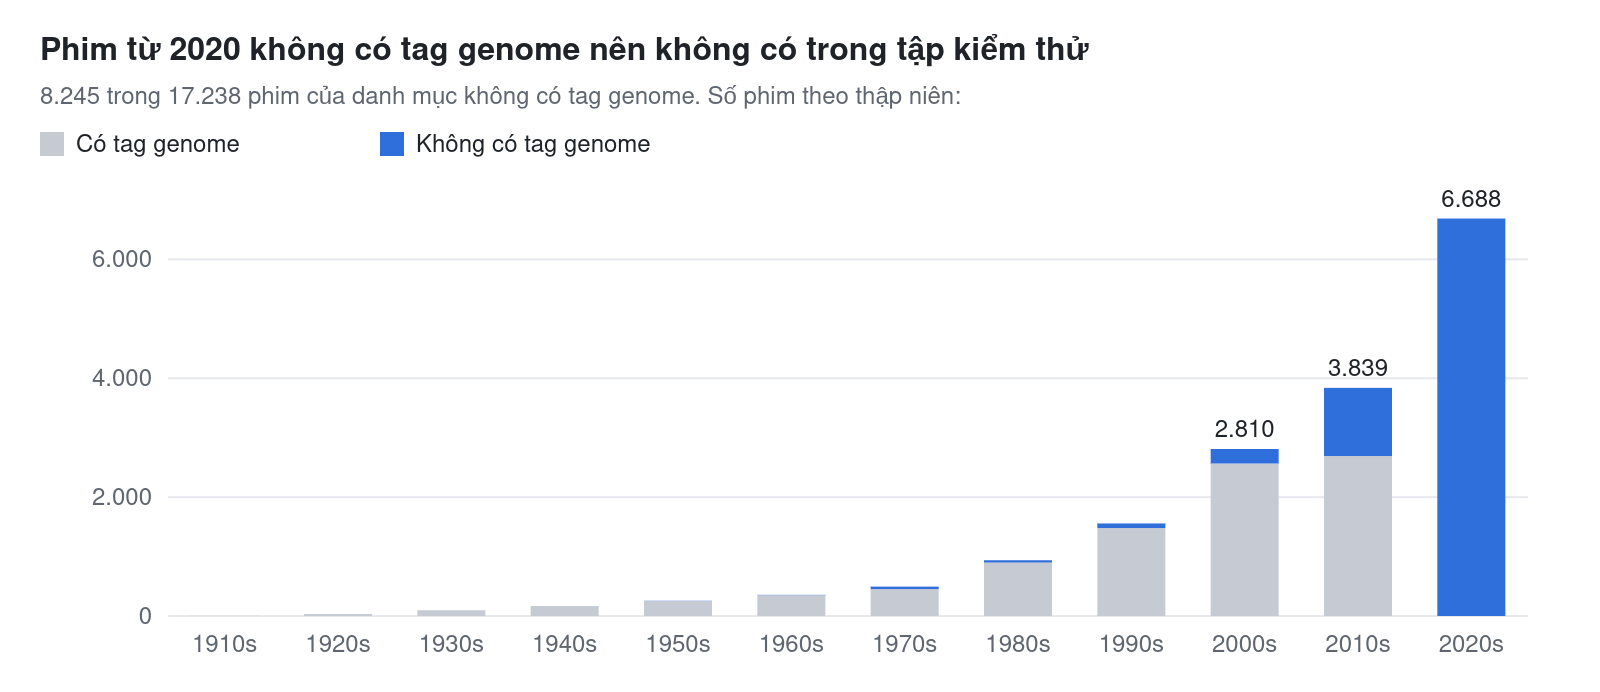
\includegraphics[width=6.26042in,height=2.70833in]{./ed07e36e8482e3fe4d0efb8173273ac4ebb13f72.png}

\emph{data/moviebot.db, đếm ngày 12/11/2026 $\cdot$ 17.238 phim}

\textbf{Hình 3.1. Số phim trong danh mục theo thập niên}
\end{figure}

Danh mục có nhiều phim từ 2020 vì ngưỡng lượt đánh giá cho phim mới thấp hơn (2.000 so với 10.000). Tag genome của MovieLens 25M dừng ở năm 2019, nên tập kiểm thử chỉ gồm phim 1920--2019.

\begin{figure}[!htbp]
\centering
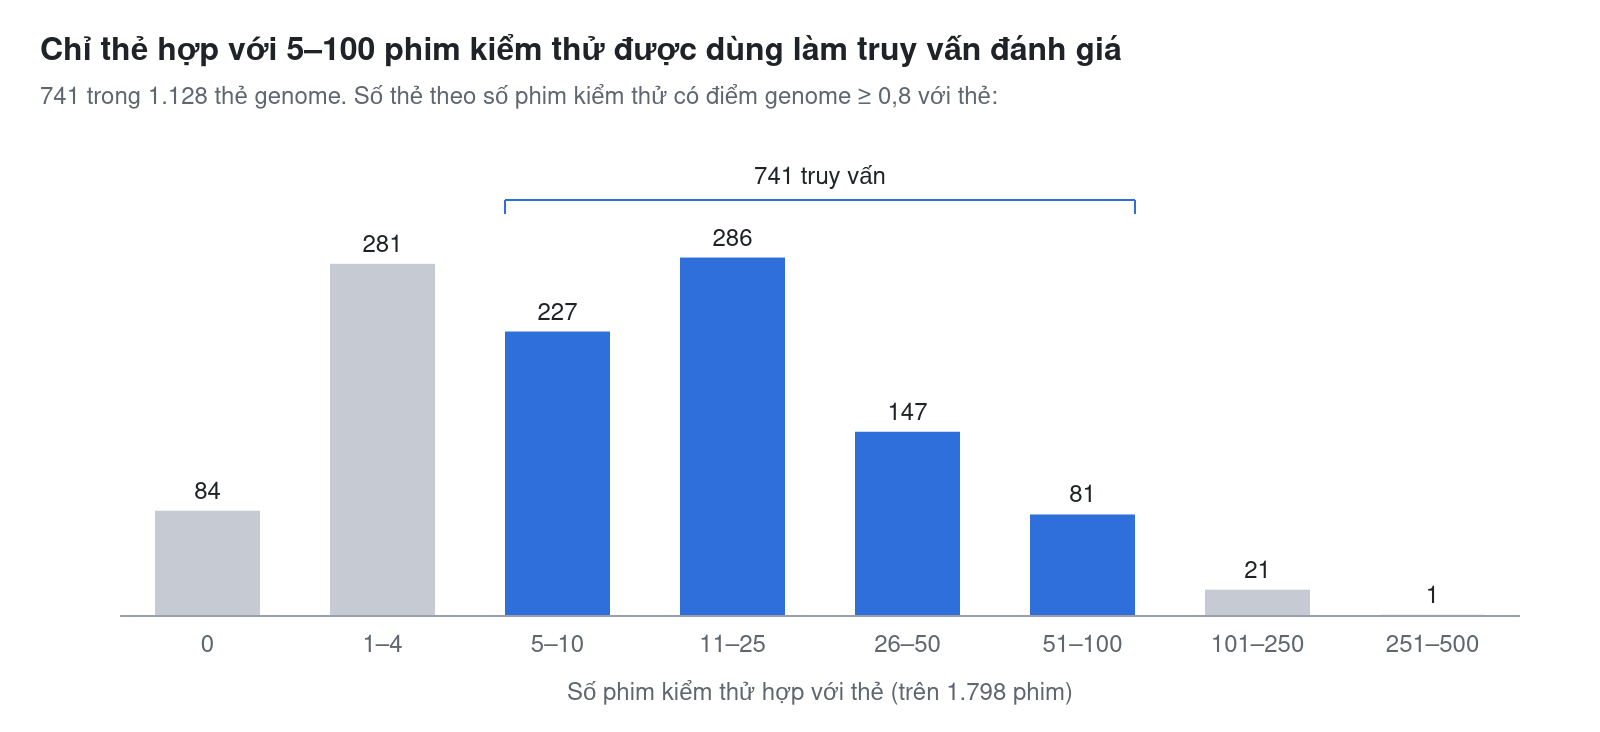
\includegraphics[width=6.26042in,height=2.86458in]{./53c01e87fd2b5ef87ee99177fb133e3b44b3c91c.png}

\emph{data/moviebot.db, chia tập seed 42, đếm ngày 12/11/2026 $\cdot$ 1.128 thẻ genome, 1.798 phim kiểm thử}

\textbf{Hình 3.2. Phân bố thẻ genome theo số phim kiểm thử phù hợp}
\end{figure}

Phân bố có đuôi dài: 365 thẻ hợp với dưới 5 phim kiểm thử, 22 thẻ hợp với hơn 100 phim.

\textbf{Mất cân bằng.} Nhóm không oversampling hay undersampling khi huấn luyện. Thẻ phổ biến vì vậy xuất hiện trong nhiều cặp hơn. Khi đánh giá, chỉ dùng 741 thẻ hợp với 5--100 phim kiểm thử. Thẻ hợp với ít hơn 5 phim cho P@10 nhiễu. Thẻ hợp với hơn 100 phim là những từ như ``original'' mà người dùng không tìm.

\subsection{2. Triển khai thực nghiệm}

\subsubsection{2.1. Môi trường}

\begin{itemize}
\tightlist
\item Huấn luyện: Google Colab, GPU T4, notebook notebooks/finetune\_search.ipynb; lần huấn luyện thứ hai (Phần III.2.5) dùng notebooks/finetune\_search\_titles.ipynb. Python 3.13.16, PyTorch 2.14.1, Sentence-Transformers 6.2.0, Transformers 5.22.2, Datasets 5.2.0, Accelerate 1.15.0.
\item Kiểm tra lại và đo hiệu năng: máy cá nhân, CPU AMD Ryzen 7 7735HS, PyTorch dùng 8 luồng, không GPU.
\item Thử nghiệm bổ sung (Phần III.3): máy cá nhân, GPU NVIDIA RTX 2060 (6 GB), script scripts/train\_search\_local.py.
\end{itemize}

\subsubsection{2.2. Phân chia bộ dữ liệu}

Chia theo cả phim và thẻ, seed 42:

\npp\textbf{Bảng 3.2. Phân chia bộ dữ liệu}

{\def\LTcaptype{}\small
\begin{longtable}[]{@{}*{4}{P{(\linewidth - 6\tabcolsep) * \real{0.2361}}}@{}}
\toprule
\textbf{Tập} & \textbf{Phim} & \textbf{Thẻ} & \textbf{Cặp (thẻ, phim)} \\
\midrule
\endhead
\bottomrule
\endlastfoot
Huấn luyện & 15.302: mọi phim có tóm tắt trừ tập kiểm thử, gồm cả phim từ 2020 & Mọi thẻ và từ khóa không thuộc 219 khóa giữ lại & 236.365 \\
Kiểm thử & 1.798: 20\% ngẫu nhiên của 8.990 phim có tag genome và tóm tắt (1920--2019) & 741 truy vấn: 589 thẻ đã thấy, 152 thẻ chưa thấy (thuộc 219 khóa giữ lại) & --- \\
\end{longtable}
}

\begin{itemize}
\tightlist
\item Hai lệnh assert trong notebook kiểm tra không cặp huấn luyện nào chứa phim kiểm thử hoặc khóa thẻ giữ lại. Luật này áp dụng cho cả thẻ người dùng và từ khóa TMDB.
\item Không có tập validation và không dùng k-fold: siêu tham số giữ mặc định của thư viện, không dò trên tập nào, và mỗi lần huấn luyện cần GPU Colab. Riêng việc dùng cả ba nguồn cặp được quyết định sau khi xem kết quả các lần chạy thử trên cùng tập kiểm thử, nên kết quả có thể lạc quan nhẹ.
\item ``Thẻ chưa thấy'' chỉ loại được biến thể chính tả. Từ đồng nghĩa của một thẻ giữ lại vẫn có thể nằm trong dữ liệu huấn luyện.
\end{itemize}

\textbf{Công thức đánh giá.} Với mỗi thẻ $t$ dùng làm truy vấn, $R_t$ là tập phim kiểm thử có $g(d,t)\geq 0{,}8$ và $\mathrm{top}_k(t)$ là $k$ phim mô hình xếp đầu. Kết quả là trung bình trên các thẻ của mỗi nhóm:

\begin{align*}
\mathrm{P@10} &= \frac{1}{|T|}\sum_{t\in T}\frac{|\mathrm{top}_{10}(t)\cap R_t|}{10}, \\
\mathrm{R@100} &= \frac{1}{|T|}\sum_{t\in T}\frac{|\mathrm{top}_{100}(t)\cap R_t|}{|R_t|}
\end{align*}

P@10 đo phần đúng trong 10 kết quả người dùng thấy đầu tiên. R@100 đo phần phim phù hợp mà mô hình đưa được vào top 100.

\subsubsection{2.3. Cấu hình mô hình và huấn luyện}

\np\textbf{Bảng 3.3. Cấu hình mô hình và huấn luyện}

{\def\LTcaptype{}\small
\begin{longtable}[]{@{}*{2}{P{(\linewidth - 2\tabcolsep) * \real{0.4947}}}@{}}
\toprule
\textbf{Tham số} & \textbf{Giá trị} \\
\midrule
\endhead
\bottomrule
\endlastfoot
Mô hình gốc & sentence-transformers/all-MiniLM-L6-v2 (6 lớp, 384 chiều, tối đa 256 token) \\
Hàm mất mát & MultipleNegativesRankingLoss, cosine, $\sigma = 20$ \\
Kích thước lô & 64 (63 mẫu âm cho mỗi cặp) \\
Bộ lấy mẫu & no\_duplicates \\
Tốc độ học & $2\times 10^{-5}$, AdamW, warmup 10\% rồi giảm tuyến tính \\
Số epoch & 3 (3.694 bước mỗi epoch, 11.082 bước) \\
Độ chính xác số & fp16 \\
Seed & 42 \\
\end{longtable}
}

\begin{figure}[!htbp]
\centering
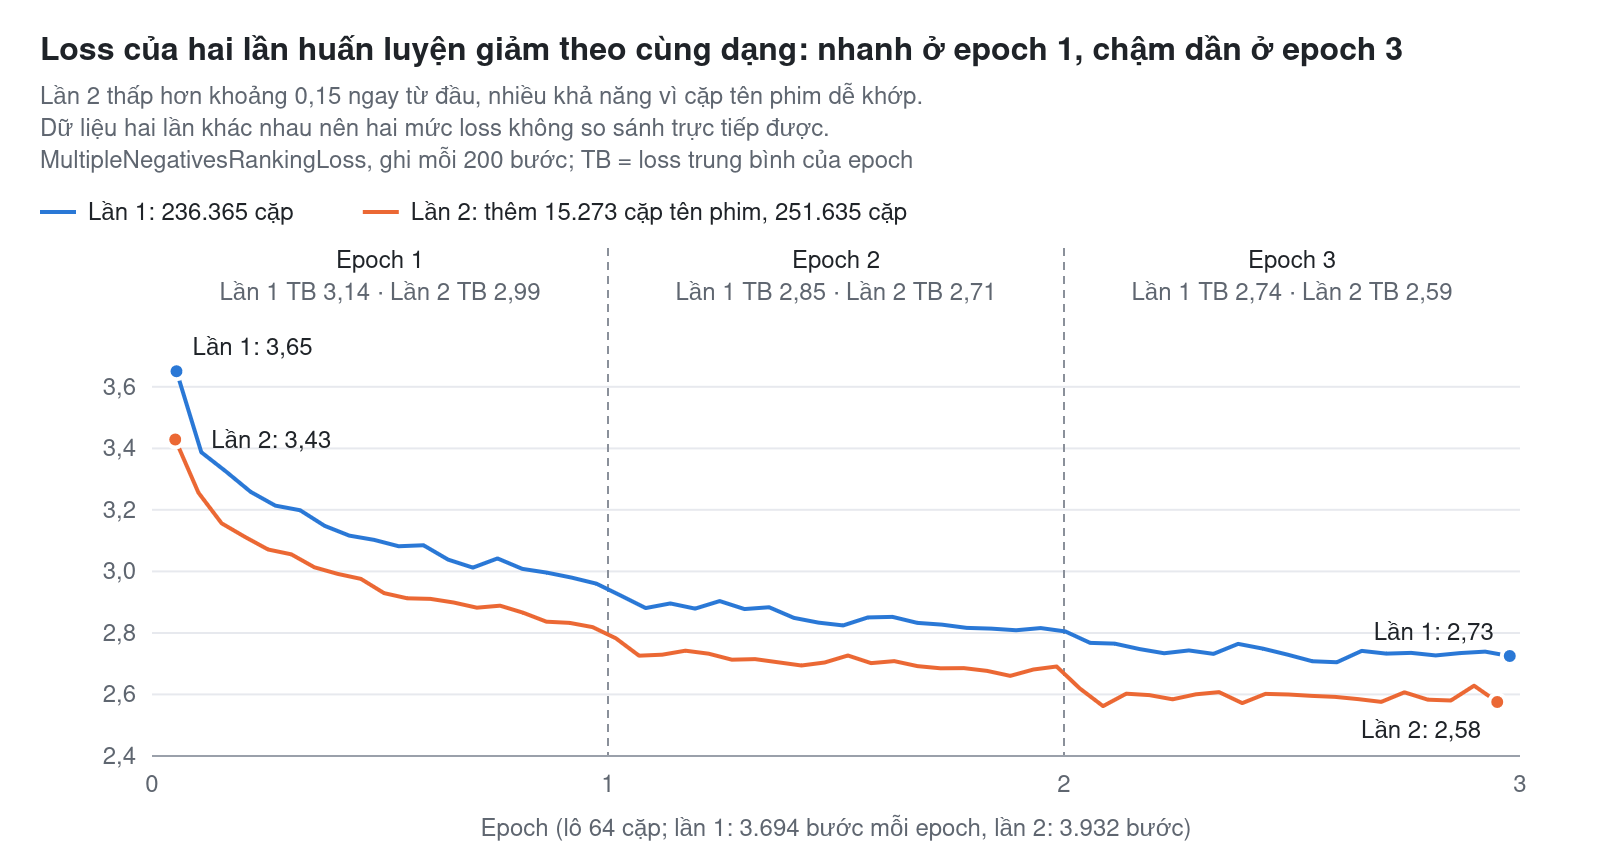
\includegraphics[width=6.26042in,height=3.38542in]{./dd7af37aff91b81d7d2e8850c01f2c355071a828.png}

\emph{data/minilm-movie-search/README.md và data/minilm-movie-search-titles/README.md (Training Logs) $\cdot$ 55 và 58 điểm ghi, Colab T4}

\textbf{Hình 3.3. Loss khi huấn luyện, lần 1 và lần 2}
\end{figure}

Ở cả hai lần, loss vẫn giảm nhẹ ở epoch 3. Lần 2 (Phần III.2.5) thấp hơn lần 1 khoảng 0,15 ở mọi epoch, nhưng dữ liệu hai lần khác nhau nên đây không phải bằng chứng mô hình lần 2 tốt hơn. Không có tập validation nên không xác định được mô hình đã bắt đầu quá khớp hay chưa.

\subsubsection{2.4. Kết quả và đánh giá}

\np\textbf{Bảng 3.4. Kết quả chính} (data/minilm-movie-search/results.json). Chạy lại phần đánh giá trên CPU ngày 12/11/2026 cho kết quả trùng đến 3 chữ số thập phân.

{\def\LTcaptype{}\small
\begin{longtable}[]{@{}*{5}{P{(\linewidth - 8\tabcolsep) * \real{0.1844}}}@{}}
\toprule
\textbf{Mô hình} & \textbf{P@10 thẻ đã thấy (589)} & \textbf{R@100 thẻ đã thấy} & \textbf{P@10 thẻ chưa thấy (152)} & \textbf{R@100 thẻ chưa thấy} \\
\midrule
\endhead
\bottomrule
\endlastfoot
BM25 & 18,1\% & 20,4\% & 14,9\% & 18,5\% \\
MiniLM gốc & 19,7\% & 36,3\% & 17,5\% & 34,2\% \\
\textbf{MiniLM tinh chỉnh} & \textbf{38,3\%} & \textbf{65,3\%} & \textbf{30,8\%} & \textbf{56,4\%} \\
\end{longtable}
}

\npp\textbf{Bảng 3.5. Các lần chạy theo lượng và nguồn dữ liệu.} Cùng tập kiểm thử. Hai lần đầu là chạy thử trên CPU (notebook với MAX\_PAIRS = 20000, EPOCHS = 1) và chỉ ghi lại P@10.

{\def\LTcaptype{}\small
\begin{longtable}[]{@{}*{6}{P{(\linewidth - 10\tabcolsep) * \real{0.1499}}}@{}}
\toprule
\textbf{Lần} & \textbf{Nguồn cặp} & \textbf{Số cặp} & \textbf{Epoch} & \textbf{P@10 thẻ đã thấy} & \textbf{P@10 thẻ chưa thấy} \\
\midrule
\endhead
\bottomrule
\endlastfoot
1 & Tag genome + thẻ người dùng & 20.000 & 1 & 29,9\% & 27,0\% \\
2 & Từ khóa TMDB & 20.000 & 1 & 27,5\% & 25,1\% \\
3 & Cả ba nguồn & 236.365 & 3 & 38,3\% & 30,8\% \\
4 & Cả ba nguồn + tên phim (Phần III.2.5) & 251.635 & 3 & 38,0\% & 30,1\% \\
\end{longtable}
}

\np\textbf{Bảng 3.6. Ví dụ truy vấn: MiniLM gốc và tinh chỉnh} (top 3, chỉ tìm trong 1.798 phim kiểm thử; 3 truy vấn cuối là tên phim chọn ngẫu nhiên với seed 42):

{\def\LTcaptype{}\small
\begin{longtable}[]{@{}*{3}{P{(\linewidth - 4\tabcolsep) * \real{0.3223}}}@{}}
\toprule
\textbf{Truy vấn} & \textbf{MiniLM gốc} & \textbf{MiniLM tinh chỉnh} \\
\midrule
\endhead
\bottomrule
\endlastfoot
twist ending & Oliver Twist; Cliffhanger; Tie Me Up! Tie Me Down! & Exam; Dream House; The Gift \\
feel-good & I Feel Pretty; Feeling Minnesota; As Good as It Gets & I, Daniel Blake; Central Station; The Polar Express \\
heist & Hesher; The Getaway (1994); Foolproof & The Getaway (1972); The Getaway (1994); Foolproof \\
cyberpunk & RoboCop; Untraceable; The Matrix & Eva; Untraceable; Next Gen \\
time travel & Looper; Timecop; The Visitors II & Timecop; Predestination; Looper \\
movies that make you cry & Cry-Baby; Moscow Does Not Believe in Tears; The Big Chill & The Big Chill; You Can Count on Me; Postcards from the Edge \\
Cracks & \textbf{Cracks}; The Mirror Crack\textquotesingle d; Shattered & Trespass; The Mirror Crack\textquotesingle d; Michael Clayton \\
Young Frankenstein & \textbf{Young Frankenstein}; Frankenstein Meets the Wolf Man; Young Adam & Frankenstein Meets the Wolf Man; \textbf{Young Frankenstein}; Nosferatu the Vampyre \\
Jane Eyre & \textbf{Jane Eyre}; The Woman in the Window; Laura & \textbf{Jane Eyre}; Austenland; Diary of a Chambermaid \\
\end{longtable}
}

\np\textbf{Bảng 3.7. Hiệu năng khi chạy} (CPU Ryzen 7 7735HS, danh mục 17.238 phim):

{\def\LTcaptype{}\small
\begin{longtable}[]{@{}*{2}{P{(\linewidth - 2\tabcolsep) * \real{0.4947}}}@{}}
\toprule
\textbf{Chỉ số} & \textbf{Giá trị} \\
\midrule
\endhead
\bottomrule
\endlastfoot
Kích thước mô hình & 90,9 MB (fp32, khoảng 22,7 triệu tham số) \\
Vector của cả danh mục & 26,5 MB ($17.238 \times 384 \times 4$ byte) \\
Nhúng cả danh mục khi khởi động & 139,8 giây \\
Độ trễ một truy vấn (mã hóa + nhân ma trận + sắp xếp, 200 truy vấn) & Trung vị 90,1 ms; p95 95,4 ms \\
\end{longtable}
}

\lbl{Nhận xét}

\begin{itemize}
\tightlist
\item Tinh chỉnh gần gấp đôi P@10 với thẻ đã thấy (+94\%) và tăng 76\% với thẻ chưa thấy. Phần lớn mức tăng vì vậy không phải do học thuộc danh sách thẻ. Khoảng cách 7,5 điểm giữa hai nhóm là phần phụ thuộc vào thẻ đã học.
\item R@100 tăng từ 36,3\% lên 65,3\%: mô hình đưa được gần hai phần ba số phim phù hợp vào top 100.
\item BM25 thấp nhất, R@100 chỉ 20,4\%: từ của thẻ thường không có trong tóm tắt phim.
\item Với cùng 20.000 cặp, thẻ MovieLens cho kết quả cao hơn từ khóa TMDB 2,4 điểm (thẻ đã thấy) và 1,9 điểm (thẻ chưa thấy). Đáp án cũng lấy từ MovieLens nên phép so sánh này có thể thiên về thẻ MovieLens. Gộp cả ba nguồn và huấn luyện 3 epoch cho kết quả cao nhất.
\item Ví dụ cho thấy mô hình tinh chỉnh hết khớp theo chữ bề mặt (``twist ending'' không còn ra Oliver Twist). Nhưng tìm theo tên phim kém hơn: ``Cracks'' không còn trong top 5, ``Young Frankenstein'' xuống vị trí 2. Mô hình đã học đọc truy vấn như một thẻ nội dung. Lần huấn luyện thứ hai sửa một phần lỗi này (Phần III.2.5).
\item Đáp án là ngưỡng 0,8 trên điểm genome (do máy dự đoán). Phim hợp với thẻ nhưng điểm dưới 0,8 bị tính là sai, nên P@10 tuyệt đối thấp hơn thực tế.
\item Huấn luyện trên Colab với GPU T4 mất khoảng 34 phút.
\item Độ trễ 90 ms trên CPU đạt yêu cầu dưới 1 giây. Khởi động mất 140 giây vì phải nhúng lại cả danh mục.
\end{itemize}

\lbl{Đề xuất cải tiến}

\begin{enumerate}
\def\labelenumi{\arabic{enumi}.}
\tightlist
\item Kết hợp tìm theo tên: khớp tên chính xác hoặc gần đúng trước, rồi mới xếp theo vector. Cách này sửa lỗi tìm theo tên.
\item Che mẫu âm sai trong lô: bỏ khỏi mẫu số những phim khác trong lô cũng hợp với thẻ (theo genome hoặc từ khóa).
\item Thêm mẫu âm khó: phim được xếp cao nhưng không hợp với thẻ (đã thử sơ bộ ở Phần III.3).
\item Tách tập validation để chọn số epoch và tốc độ học mà không dùng tập kiểm thử. Giới hạn số cặp của mỗi thẻ để giảm lệch về thẻ phổ biến.
\item Lưu vector danh mục ra đĩa để khởi động trong vài giây. Dùng chỉ mục ANN (FAISS, HNSW) nếu danh mục tăng lên hàng triệu phim.
\item Dùng mô hình đa ngôn ngữ (ví dụ paraphrase-multilingual-MiniLM-L12-v2) để nhận truy vấn tiếng Việt.
\end{enumerate}

\subsubsection{2.5. Lần huấn luyện thứ hai: thêm cặp tên phim}

Mô hình ở Phần III.2.4 tìm theo tên phim kém. Lần huấn luyện thứ hai thêm cho mỗi phim huấn luyện một cặp (tên phim, văn bản phim) và giữ nguyên mọi thứ khác.

\lbl{Thay đổi so với lần 1}

\begin{itemize}
\tightlist
\item Notebook notebooks/finetune\_search\_titles.ipynb: cùng seed, cùng cách chia tập, cùng cấu hình ở Phần III.2.3.
\item 15.273 cặp tên phim, chỉ lấy từ phim huấn luyện. Bỏ tên trùng với một khóa thẻ giữ lại (ví dụ phim tên ``Heist'') để thẻ chưa thấy vẫn chưa thấy. Gộp với 236.365 cặp cũ và bỏ trùng còn 251.635 cặp, 3.932 bước mỗi epoch. Hai lệnh assert kiểm tra rò rỉ vẫn đạt.
\item Thêm phép kiểm thử tên phim: tìm tên của 1.798 phim kiểm thử trong cả danh mục. Mô hình chưa học tên các phim này. hit@1 là tỉ lệ truy vấn có phim mang đúng tên đó đứng đầu; phim làm lại cùng tên cũng tính là đúng. hit@10 tính tương tự trên top 10.
\end{itemize}

\textbf{Kết hợp với BM25.} Nhóm thử thêm cách ghép danh sách của MiniLM và BM25 bằng Reciprocal Rank Fusion (RRF). $r$ là thứ hạng của phim trong top 100 của mỗi danh sách; phim không có trong một danh sách nhận 0 điểm từ danh sách đó:

\[
\mathrm{RRF}(d)=\frac{1}{60+r_{\mathrm{MiniLM}}(d)}+\frac{1}{60+r_{\mathrm{BM25}}(d)}
\]

Hằng số 60 là giá trị mặc định thường dùng, không dò trên tập kiểm thử.

\np\textbf{Bảng 3.8. Kết quả lần huấn luyện thứ hai và RRF} (chạy trên CPU ngày 13/11/2026). P@10 và R@100 đo trên 1.798 phim kiểm thử như Phần III.2.4. Tên phim được tìm trong cả 17.238 phim của danh mục, như trên trang demo.

{\def\LTcaptype{}\footnotesize
\begin{longtable}[]{@{}*{7}{P{(\linewidth - 12\tabcolsep) * \real{0.1252}}}@{}}
\toprule
\textbf{Mô hình} & \textbf{P@10 thẻ đã thấy (589)} & \textbf{R@100 thẻ đã thấy} & \textbf{P@10 thẻ chưa thấy (152)} & \textbf{R@100 thẻ chưa thấy} & \textbf{Tên phim hit@1 (1.798)} & \textbf{Tên phim hit@10} \\
\midrule
\endhead
\bottomrule
\endlastfoot
BM25 & 18,1\% & 20,4\% & 14,9\% & 18,5\% & 70,4\% & 92,5\% \\
MiniLM gốc & 19,7\% & 36,3\% & 17,5\% & 34,2\% & 88,6\% & 99,0\% \\
Tinh chỉnh lần 1 & 38,3\% & 65,3\% & 30,8\% & 56,4\% & 27,0\% & 52,6\% \\
\textbf{Tinh chỉnh lần 2 (thêm tên phim)} & \textbf{38,0\%} & \textbf{64,9\%} & \textbf{30,1\%} & \textbf{55,9\%} & \textbf{62,5\%} & \textbf{91,7\%} \\
Lần 1 + BM25 (RRF) & 34,5\% & 63,4\% & 28,3\% & 55,2\% & 48,3\% & 86,3\% \\
Lần 2 + BM25 (RRF) & 34,4\% & 62,7\% & 28,1\% & 54,9\% & 76,9\% & 97,3\% \\
\end{longtable}
}

\begin{itemize}
\tightlist
\item results.json của lần 2 (chạy trên Colab) cho cùng P@10 và R@100. Hit@1 tên phim trong notebook là 63,5\% vì notebook chỉ tìm trong 17.100 phim có tóm tắt.
\item Trên 1.000 tên chọn ngẫu nhiên từ cả danh mục, gần với truy vấn thật trên trang demo, hit@1 là 72,7\% (lần 2), 29,5\% (lần 1) và 88,8\% (mô hình gốc). Phần lớn các tên này thuộc phim huấn luyện mà lần 2 đã học, nên con số cao hơn trên tập kiểm thử.
\item Lần 2 cùng kiến trúc và kích thước với lần 1, nên độ trễ và bộ nhớ như Phần III.2.4 (không đo lại).
\end{itemize}

\np\textbf{Bảng 3.9. Độ tin cậy của chênh lệch P@10} (khoảng tin cậy 95\%, bootstrap 10.000 lần trên các truy vấn):

{\def\LTcaptype{}\small
\begin{longtable}[]{@{}*{3}{P{(\linewidth - 4\tabcolsep) * \real{0.3223}}}@{}}
\toprule
\textbf{So sánh} & \textbf{Thẻ đã thấy} & \textbf{Thẻ chưa thấy} \\
\midrule
\endhead
\bottomrule
\endlastfoot
Lần 2 so với lần 1 & \mn 0,2 điểm {[}\mn 0,8; +0,4{]} & \mn 0,7 điểm {[}\mn 1,9; +0,6{]} \\
Lần 2 + BM25 so với lần 2 & \mn 3,7 điểm {[}\mn 4,7; \mn 2,6{]} & \mn 2,0 điểm {[}\mn 3,9; \mn 0,3{]} \\
\end{longtable}
}

\Needspace{20\baselineskip}\textbf{Bảng 3.10. Ví dụ truy vấn: lần 1 và lần 2} (top 3, tìm trong cả 17.238 phim):

{\def\LTcaptype{}\small
\begin{longtable}[]{@{}*{3}{P{(\linewidth - 4\tabcolsep) * \real{0.3223}}}@{}}
\toprule
\textbf{Truy vấn} & \textbf{Tinh chỉnh lần 1} & \textbf{Tinh chỉnh lần 2} \\
\midrule
\endhead
\bottomrule
\endlastfoot
the godfather & The Godfather Part II; \textbf{The Godfather}; The Godfather Part III & \textbf{The Godfather}; The Godfather Part II; The Godfather Part III \\
alien & Meet Dave; The Cabbage Soup; Alien: Romulus & Meet Dave; The Cabbage Soup; Alien: Romulus \\
young frankenstein & Mary Shelley\textquotesingle s Frankenstein; Frankenstein (2025); The Curse of Frankenstein & Frankenstein (2025); Mary Shelley\textquotesingle s Frankenstein; The Bride! \\
feel-good & I, Daniel Blake; My King; Central Station & I Feel Pretty; Now Is Good; The Fundamentals of Caring \\
twist ending & Secret Window; The I Inside; Amusement & Secret Window; Twisted; The I Inside \\
heist & American Heist; The Getaway (1972); The Getaway (1994) & American Heist; Heist (2001); World Cup Heist \\
\end{longtable}
}

\lbl{Nhận xét}

\begin{itemize}
\tightlist
\item Cặp tên phim chiếm khoảng 6\% dữ liệu và không làm giảm chất lượng tìm theo nội dung: khoảng tin cậy của chênh lệch P@10 giữa lần 2 và lần 1 chứa 0.
\item Tỉ lệ tên phim đứng đầu tăng từ 27,0\% lên 62,5\%, tỉ lệ có trong top 10 từ 52,6\% lên 91,7\%. Tên của phim kiểm thử không có trong dữ liệu huấn luyện, nên mô hình học được cách khớp tên, không chỉ nhớ tên đã thấy.
\item Lần 2 vẫn kém mô hình gốc (88,6\%) và BM25 (70,4\%) khi tìm theo tên. Phim đúng thường nằm trong top 10 nhưng không đứng đầu. Lỗi rõ nhất là tên một từ trùng với chủ đề: ``alien'' trả về \emph{Meet Dave}, một phim về người ngoài hành tinh, thay vì \emph{Alien} (1979). \emph{Young Frankenstein} (phim kiểm thử) không có trong top 5 ở cả hai lần.
\item Một vài ví dụ có lại khớp chữ bề mặt (``feel-good'' ra \emph{I Feel Pretty}, ``twist ending'' ra \emph{Twisted}), nhưng P@10 trên 741 truy vấn thẻ không đổi.
\item Ghép với BM25 bằng RRF nâng hit@1 tên phim lên 76,9\% nhưng giảm P@10 3,7 điểm (thẻ đã thấy) và 2,0 điểm (thẻ chưa thấy) so với lần 2 dùng riêng; cả hai mức giảm nằm ngoài sai số. BM25 đưa lại các phim khớp chữ bề mặt. Phần III.2.6 giảm trọng số của BM25 để giữ P@10.
\item Lần 2 ngang lần 1 về tìm theo nội dung và tốt hơn rõ rệt về tìm theo tên. Trang demo chạy mô hình lần 2 ghép BM25 (Phần III.2.6); ảnh cuối ở Phụ lục D chụp với mô hình lần 2 trước khi ghép BM25.
\item Chưa thử: khớp tên chính xác trước (đề xuất 1 ở Phần III.2.4), lặp lại cặp tên phim nhiều lần khi huấn luyện. Trọng số BM25 thấp hơn được thử ở Phần III.2.6. Chưa đo với tên gõ sai hoặc chỉ gõ một phần tên.
\end{itemize}

\subsubsection{2.6. Ghép với BM25 theo trọng số (mô hình trên trang demo)}

RRF ở Phần III.2.5 cho MiniLM và BM25 cùng trọng số nên làm giảm P@10. Search API (notebooks/search\_site.py) ghép hai danh sách với trọng số 0,8 cho MiniLM và 0,2 cho BM25:

\[
s(d)=\frac{0{,}8}{60+r_{\mathrm{MiniLM}}(d)}+\frac{0{,}2}{60+r_{\mathrm{BM25}}(d)}
\]

\begin{itemize}
\tightlist
\item $r$ là thứ hạng của phim trong cả danh mục. Phim không chứa từ nào của truy vấn không nhận điểm BM25.
\item BM25 dùng thư viện rank\_bm25 (BM25Okapi, $k_1 = 1{,}5$, $b = 0{,}75$), tách từ bằng \textbackslash w+ trên chữ thường, không đưa từ về gốc. Bản này khác bản FTS5 ở Phần II.2.1, nên số liệu BM25 lệch nhẹ so với các phần trước.
\item Trọng số 0,2 được chọn sau khi xem kết quả trên tập kiểm thử. Bảng dưới thử thêm 0,1, 0,3 và 0,5 để xem kết quả phụ thuộc vào trọng số đến mức nào. Trọng số 0,5 cho cùng công thức với RRF ở Phần III.2.5, khác bản BM25.
\end{itemize}

\np\textbf{Bảng 3.11. Kết quả ghép BM25 theo trọng số} (notebooks/hybrid\_eval.py, chạy trên CPU ngày 16/11/2026). Cùng tập kiểm thử và cách tính như Phần III.2.5. Tên phim được tìm trong 17.100 phim có tóm tắt như notebook, nên mô hình lần 2 dùng riêng đạt hit@1 63,5\% thay vì 62,5\% ở Phần III.2.5.

{\def\LTcaptype{}\footnotesize
\begin{longtable}[]{@{}*{8}{P{(\linewidth - 14\tabcolsep) * \real{0.1068}}}@{}}
\toprule
\textbf{Mô hình} & \textbf{Trọng số BM25} & \textbf{P@10 thẻ đã thấy (589)} & \textbf{R@100 thẻ đã thấy} & \textbf{P@10 thẻ chưa thấy (152)} & \textbf{R@100 thẻ chưa thấy} & \textbf{Tên phim hit@1 (1.798)} & \textbf{Tên phim hit@10} \\
\midrule
\endhead
\bottomrule
\endlastfoot
BM25 (rank\_\allowbreak bm25) & --- & 16,4\% & 19,8\% & 14,6\% & 19,5\% & 73,4\% & 94,8\% \\
Tinh chỉnh lần 1 & 0 & 38,3\% & 65,3\% & 30,8\% & 56,4\% & 27,1\% & 52,7\% \\
Lần 1 + BM25 & 0,2 & 38,8\% & 65,4\% & 31,2\% & 56,9\% & 40,8\% & 63,0\% \\
Tinh chỉnh lần 2 & 0 & 38,0\% & 64,9\% & 30,1\% & 55,9\% & 63,5\% & 91,8\% \\
Lần 2 + BM25 & 0,1 & 38,4\% & 65,0\% & 30,3\% & 56,2\% & 73,2\% & 94,1\% \\
\textbf{Lần 2 + BM25 (trang demo)} & \textbf{0,2} & \textbf{38,4\%} & \textbf{64,9\%} & \textbf{30,5\%} & \textbf{56,3\%} & \textbf{75,6\%} & \textbf{95,7\%} \\
Lần 2 + BM25 & 0,3 & 37,7\% & 64,3\% & 29,5\% & 56,0\% & 77,3\% & 97,1\% \\
Lần 2 + BM25 & 0,5 & 32,7\% & 62,8\% & 26,7\% & 54,7\% & 79,7\% & 98,4\% \\
\end{longtable}
}

\Needspace{17\baselineskip}\textbf{Bảng 3.12. Độ tin cậy của chênh lệch so với lần 2 dùng riêng} (điểm phần trăm, khoảng tin cậy 95\%, bootstrap 10.000 lần trên các truy vấn). Cột cuối: số truy vấn tên phim mà bản ghép đưa phim đúng lên đầu trong khi lần 2 dùng riêng thì không (sửa), và ngược lại (hỏng).

{\def\LTcaptype{}\small
\begin{longtable}[]{@{}*{5}{P{(\linewidth - 8\tabcolsep) * \real{0.1844}}}@{}}
\toprule
\textbf{Trọng số BM25} & \textbf{P@10 thẻ đã thấy} & \textbf{P@10 thẻ chưa thấy} & \textbf{Tên phim hit@1} & \textbf{Sửa / hỏng} \\
\midrule
\endhead
\bottomrule
\endlastfoot
0,1 & +0,3 {[}0,0; +0,7{]} & +0,1 {[}\mn 0,5; +0,8{]} & +9,7 {[}+8,3; +11,2{]} & 182 / 7 \\
0,2 & +0,3 {[}\mn 0,2; +0,9{]} & +0,3 {[}\mn 0,6; +1,2{]} & +12,1 {[}+10,5; +13,7{]} & 235 / 18 \\
0,3 & \mn 0,4 {[}\mn 1,1; +0,4{]} & \mn 0,7 {[}\mn 1,8; +0,6{]} & +13,8 {[}+12,0; +15,6{]} & 282 / 34 \\
0,5 & \mn 5,3 {[}\mn 6,5; \mn 4,2{]} & \mn 3,4 {[}\mn 5,3; \mn 1,6{]} & +16,2 {[}+14,1; +18,3{]} & 359 / 68 \\
\end{longtable}
}

\textbf{Hit@1 tăng ở đâu} (trọng số 0,2). Trong 235 truy vấn được sửa, MiniLM đã xếp phim đúng ở vị trí 2 trong 117 truy vấn, 3--5 trong 83, 6--20 trong 32. BM25 xếp phim đúng thứ nhất trong 175 truy vấn. Phim BM25 xếp thứ nhất được cộng $0{,}2/61 \approx 0{,}0033$ điểm. Nếu phim MiniLM xếp đầu không chung từ nào với truy vấn, phim kia vượt lên khi nằm trong top 21 của MiniLM, vì $0{,}8/(60+r) + 0{,}2/61 > 0{,}8/61$ khi $r \leq 21$.

\np\textbf{Bảng 3.13. Ví dụ truy vấn tên phim được sửa và bị hỏng} (hạng tính trên 17.100 phim; phim đứng đầu khi sai là của lần 2 dùng riêng với dòng ``Sửa'', của bản ghép với dòng ``Hỏng''):

{\def\LTcaptype{}\small
\begin{longtable}[]{@{}*{5}{P{(\linewidth - 8\tabcolsep) * \real{0.1844}}}@{}}
\toprule
\textbf{Truy vấn} & \textbf{Thay đổi} & \textbf{Phim đúng: hạng MiniLM / BM25} & \textbf{Phim đứng đầu khi sai} & \textbf{Phim đó: hạng MiniLM / BM25} \\
\midrule
\endhead
\bottomrule
\endlastfoot
The China Syndrome (1979) & Sửa & 2 / 1 & Sight (2023) & 1 / 40 \\
Pandorum (2009) & Sửa & 2 / 1 & Pani (2024) & 1 / không chung từ \\
The Secret of NIMH (1982) & Sửa & 7 / 1 & Nindha (2024) & 1 / 12.954 \\
Porco Rosso (1992) & Sửa & 8 / 1 & Don Juan DeMarco (1994) & 1 / không chung từ \\
Little White Lies (2010) & Sửa & 2 / 1 & A Little White Lie (2023) & 1 / 6 \\
Michael (1996) & Hỏng & 1 / 29 & Finding Michael (2023) & 2 / 7 \\
Next (2007) & Hỏng & 1 / 261 & Girl Next (2021) & 2 / 5 \\
High School Musical 2 (2007) & Hỏng & 1 / 9 & High School Musical 3: Senior Year (2008) & 2 / 3 \\
\end{longtable}
}

\lbl{Nhận xét}

\begin{itemize}
\tightlist
\item Trọng số 0,1--0,3 giữ P@10 trong sai số (khoảng tin cậy chứa 0) và tăng hit@1 tên phim 9,7--13,8 điểm, nên kết quả không phụ thuộc vào việc chọn đúng 0,2. Trọng số 0,5 giảm P@10 5,3 điểm (thẻ đã thấy) và 3,4 điểm (thẻ chưa thấy), cùng chiều với Phần III.2.5.
\item Phần lớn mức tăng đến từ truy vấn mà MiniLM đã đưa phim đúng vào top 5 nhưng xếp trước nó một phim có tên gần giống về âm (Pani, Nindha) hoặc không chung từ nào với truy vấn. Với trọng số 0,2, một phim chỉ vào được top 10 của bản ghép khi MiniLM xếp nó trong top 38 ($0{,}8/(60+r) + 0{,}2/61 \geq 0{,}8/70$ khi $r \leq 38$). BM25 chỉ sắp xếp lại các phim MiniLM đã xếp cao.
\item Truy vấn bị hỏng là tên ngắn, phổ biến (Michael, Next) hoặc phim nhiều phần (High School Musical 2): một phim có tên dài hơn chứa cùng từ đứng ngay sau phim đúng trong MiniLM và được BM25 xếp cao hơn.
\item Lần 1 + BM25 0,2 có P@10 cao hơn lần 2 + BM25 0,2 (0,4 và 0,7 điểm), cùng cỡ với chênh lệch lần 1 -- lần 2 ở Phần III.2.5 vốn nằm trong sai số, nhưng hit@1 tên phim chỉ 40,8\% so với 75,6\%. Lần 2 + BM25 0,2 là phương án tốt nhất trong các phương án đã thử.
\item Hit@1 vẫn thấp hơn MiniLM gốc (88,7\% trong notebook). Trên cả danh mục 17.238 phim, ``Heat'', ``Alien'', ``Up'' và ``Her'' vẫn không có phim đúng trong top 5, với cả lần 2 dùng riêng và bản ghép.
\item Hiệu năng (CPU Ryzen 7 7735HS, 17.238 phim, 200 truy vấn gồm 100 thẻ genome và 100 tên phim chọn ngẫu nhiên): độ trễ trung vị 88,8 ms, p95 113,4 ms; khởi động (nhúng danh mục và lập chỉ mục BM25) 141,7 giây. Phần III.2.4 đo MiniLM dùng riêng với bộ truy vấn khác: trung vị 90,1 ms, p95 95,4 ms.
\end{itemize}

\subsection{3. Thử nghiệm bổ sung: hard negatives}

Đây là thử nghiệm thăm dò theo đề xuất 3 ở Phần III.2.4; mô hình chính và trang demo không thay đổi.

Mô hình làm mốc là \textbf{MiniLM tinh chỉnh lần 1} (236.365 cặp, Phần III.2.3--2.4), không phải MiniLM gốc. Nhóm huấn luyện tiếp mô hình này với \textit{mẫu âm khó} (hard negatives): phim mà mô hình dễ nhầm là hợp với thẻ nhưng có điểm tag genome thấp.

\begin{itemize}
\tightlist
\item Với mỗi thẻ trong tập huấn luyện, dùng mô hình lần 1 lấy top 100 phim, chỉ trong các phim huấn luyện. Không dùng phim kiểm thử hoặc khóa thẻ giữ lại.
\item Mẫu đúng: phim có $g(d,t) \ge 0{,}8$. Mẫu âm khó: phim trong top 100 có $g(d,t) \le 0{,}1$. Mỗi mẫu đúng ghép với 1 mẫu âm khó thành bộ ba (thẻ, phim đúng, phim âm), tổng 36.703 bộ ba.
\item Huấn luyện thêm 1 epoch, tốc độ học $5 \times 10^{-6}$, kích thước lô 16 (giới hạn bởi 6 GB VRAM), khoảng 3 phút trên RTX 2060.
\item Top 100, ngưỡng 0,1 và 1 mẫu âm cho mỗi mẫu đúng là thiết lập ban đầu. Nhóm thử thêm cấu hình chỉ lấy mẫu âm trong top 20 (tốc độ học $2 \times 10^{-6}$); trên tập kiểm thử, cấu hình này đạt P@10 39,1\% và 32,2\% khi ghép BM25, thấp hơn top 100.
\item Để đối chiếu mà không dùng tập kiểm thử, nhóm tách 10\% phim và khóa thẻ từ tập huấn luyện làm tập validation (719 phim, 87 thẻ), huấn luyện lại mô hình lần 1 trên phần còn lại (lô 64, khoảng 18 phút) rồi chạy cả hai cấu hình. P@10 trên validation khi ghép BM25 80/20 (thẻ đã thấy / chưa thấy): mốc 37,1\% / 30,6\%; top 20: 37,1\% / 31,2\%; top 100: 38,2\% / 32,1\%. Validation cho cùng kết luận: top 100 tốt hơn.
\end{itemize}

Bảng dưới so sánh trước và sau bước này (seed 42, chưa ghép BM25), trên cùng bộ kiểm thử 1.798 phim:

\np\textbf{Bảng 3.14. So sánh trước và sau khi thêm mẫu âm khó}
{\def\LTcaptype{}\small
\begin{longtable}[]{@{}*{5}{P{(\linewidth - 8\tabcolsep) * \real{0.1844}}}@{}}
\toprule
\textbf{Mô hình} & \textbf{P@10 thẻ đã thấy (589)} & \textbf{R@100 thẻ đã thấy} & \textbf{P@10 thẻ chưa thấy (152)} & \textbf{R@100 thẻ chưa thấy} \\
\midrule
\endhead
\bottomrule
\endlastfoot
MiniLM tinh chỉnh (III.2.4) & 38,3\% & 65,3\% & 30,8\% & 56,4\% \\
\textbf{Thêm mẫu âm khó} & \textbf{39,6\%} & \textbf{66,3\%} & \textbf{33,1\%} & \textbf{57,7\%} \\
\end{longtable}
}

\Needspace{15\baselineskip}\textbf{Bảng 3.15. Kết quả mẫu âm khó qua 5 seed huấn luyện} (ghép BM25 80/20).
\begin{center}
\small
\begin{tabular}{lrrrr}
\toprule
& \multicolumn{2}{c}{\textbf{Thẻ đã thấy (589)}} & \multicolumn{2}{c}{\textbf{Thẻ chưa thấy (152)}} \\
\cmidrule(lr){2-3} \cmidrule(lr){4-5}
\textbf{Cấu hình} & \textbf{P@10} & \textbf{R@100} & \textbf{P@10} & \textbf{R@100} \\
\midrule
Lần 1 (mốc) & 38,7\% & 65,4\% & 31,4\% & 56,9\% \\
Seed 42 & 40,4\% & 66,5\% & 33,6\% & 58,3\% \\
Seed 43 & 40,4\% & 66,7\% & 33,9\% & 58,7\% \\
Seed 44 & 40,3\% & 66,4\% & 33,9\% & 57,9\% \\
Seed 45 & 40,4\% & 66,6\% & 34,4\% & 58,4\% \\
Seed 46 & 40,3\% & 66,7\% & 34,1\% & 58,1\% \\
\textbf{Trung bình} & \textbf{40,4\%} & \textbf{66,6\%} & \textbf{34,0\%} & \textbf{58,3\%} \\
\bottomrule
\end{tabular}
\end{center}
Dòng mốc là mô hình lần 1 chưa thêm mẫu âm khó; các dòng seed là sau khi thêm. Mọi dòng ghép BM25 80/20 bằng SQLite FTS5, nên dòng mốc lệch nhẹ so với dòng ``Lần 1 + BM25 0,2'' ở Bảng 3.11 (dùng rank\_bm25). Năm lần chạy giữ cùng mô hình khởi đầu, cùng bộ ba và cùng tập kiểm thử, chỉ đổi seed huấn luyện. R@100 được tính lại từ mô hình đã lưu; trung bình P@10 tính từ điểm đã làm tròn.

\Needspace{8\baselineskip}\textbf{Bảng 3.16. Ví dụ truy vấn: lần 2 và lần 1 + mẫu âm khó} (top 3, cả hai ghép BM25 80/20, tìm trong 17.097 phim có tóm tắt như trang demo; in đậm: phim có điểm tag genome $\ge 0{,}8$ với thẻ):

{\def\LTcaptype{}\small
\begin{longtable}[]{@{}*{3}{P{(\linewidth - 4\tabcolsep) * \real{0.3223}}}@{}}
\toprule
\textbf{Truy vấn} & \textbf{Tinh chỉnh lần 2 (trang demo)} & \textbf{Lần 1 + mẫu âm khó (seed 42)} \\
\midrule
\endhead
\bottomrule
\endlastfoot
heist & World Cup Heist; American Heist; Stolen: Heist of the Century & American Heist; \textbf{The Getaway (1972)}; \textbf{The Score} \\
time travel & Our Times; The Visitor from the Future; See You Yesterday & \textbf{The Time Machine (2002)}; \textbf{Timecop}; \textbf{Timecrimes} \\
serial killer & Chronicle of a Serial Killer; My Father, the BTK Killer; Artiste & \textbf{Kalifornia}; \textbf{Eyes of Laura Mars}; \textbf{Henry: Portrait of a Serial Killer} \\
dystopia & \textbf{Equilibrium}; 2073; Ganapath & \textbf{Equilibrium}; \textbf{THX 1138}; \textbf{The Hunger Games} \\
twist ending & \textbf{Twisted}; \textbf{Secret Window}; The I Inside & The I Inside; \textbf{Secret Window}; Amusement \\*
feel-good & I Feel Pretty; Feels Good Man; Now Is Good & \textbf{Pay It Forward}; American Beauty; Kids \\
\end{longtable}
}

Phim từ 2020 trở đi chưa có tag genome nên không được in đậm dù có thể phù hợp; mô hình lần 2 trả về nhiều phim loại này hơn. Danh mục gồm cả phim huấn luyện, nên bảng chỉ để minh họa.

\lbl{Nhận xét}

\begin{itemize}
\tightlist
\item Mẫu âm khó tăng P@10 khoảng 1,7 điểm với thẻ đã thấy và 2,6 điểm với thẻ chưa thấy (sau khi ghép BM25). R@100 tăng khoảng 1,2--1,4 điểm.
\item Năm seed chênh nhau không quá 0,1 điểm (thẻ đã thấy) và 0,8 điểm (thẻ chưa thấy), đều cao hơn mốc. Vậy mức tăng không phải do một seed may mắn.
\item Tập validation được chạy sau khi nhóm đã xem kết quả hai cấu hình trên tập kiểm thử, và chỉ có 87 thẻ. Validation cho cùng kết luận, nhưng vẫn cần một tập kiểm thử độc lập mới để xác nhận.
\item Ở Bảng 3.16, mô hình lần 2 hay xếp đầu những phim có từ của truy vấn ngay trong tên (World Cup Heist, Chronicle of a Serial Killer), còn mô hình có mẫu âm khó trả về phim đúng chủ đề hơn. Ngược lại, khi tìm theo tên phim, tỉ lệ phim đúng đứng đầu của mô hình mẫu âm khó chỉ 48,1\%, so với khoảng 75\% của lần 2 (Bảng 3.11).
\item Đây chỉ là thử nghiệm, không áp dụng vào trang demo; trang demo vẫn dùng mô hình lần 2 + BM25 (Phần III.2.6).
\end{itemize}

% =====================================================================
%  PHẦN IV
% =====================================================================
\chap{PHẦN IV. KẾT LUẬN}

Nhóm đã tinh chỉnh all-MiniLM-L6-v2 cho tìm kiếm phim theo từ khóa. Trên phim chưa dùng khi huấn luyện, P@10 tăng từ 19,7\% lên 38,3\%, và từ 17,5\% lên 30,8\% với thẻ chưa thấy. Lần huấn luyện thứ hai thêm cặp tên phim, giữ nguyên P@10 và nâng tỉ lệ tên phim đứng đầu kết quả từ 27,0\% lên 62,5\%. Trang demo ghép mô hình lần 2 với BM25 theo trọng số 80/20: P@10 không đổi, tỉ lệ tên phim đứng đầu tăng thêm 12,1 điểm.

\lbl{Kết quả đạt được}

\begin{itemize}
\tightlist
\item Bộ dữ liệu 236.365 cặp (thẻ, phim) xây dựng từ nhãn có sẵn của MovieLens và TMDB, không gán nhãn thủ công.
\item Quy trình chia tập theo cả phim và thẻ, có kiểm tra rò rỉ dữ liệu.
\item Mô hình vượt BM25 và mô hình gốc trên cả P@10 và R@100, kết quả tái lập được trên CPU.
\item Search API (FastAPI) và trang demo (Next.js) chạy trên CPU, độ trễ trung vị 90 ms một truy vấn.
\end{itemize}

\lbl{Hạn chế}

\begin{itemize}
\tightlist
\item Tìm theo tên phim vẫn kém mô hình gốc: tên phim đứng đầu 75,6\% số lần với mô hình lần 2 ghép BM25, so với 88,7\% của mô hình gốc (tìm trong 17.100 phim có tóm tắt, Phần III.2.6). Tên một từ trùng chủ đề (``Heat'', ``Alien'') vẫn sai.
\item Tập kiểm thử chỉ có phim đến 2019. Chưa đo được chất lượng trên 6.688 phim từ 2020.
\item Đáp án là điểm genome do máy dự đoán. Chưa có đánh giá bởi người dùng thật.
\item Các lần huấn luyện chính ở Phần III.2 không có tập validation và chưa đo độ dao động giữa các seed. Trọng số BM25 của trang demo được chọn sau khi xem kết quả trên tập kiểm thử. Thử nghiệm mẫu âm khó ở Phần III.3 chỉ được đối chiếu trên một tập validation nhỏ (87 thẻ), chạy sau khi đã xem tập kiểm thử, và chưa được xác nhận trên một tập kiểm thử độc lập mới.
\item Chỉ nhận truy vấn tiếng Anh.
\end{itemize}

\lbl{Hướng phát triển}

\begin{itemize}
\tightlist
\item Các cải tiến mô hình ở Phần III.2.4: kết hợp tìm theo tên, che mẫu âm sai, tập validation, mô hình đa ngôn ngữ. Áp dụng mẫu âm khó (đã thử sơ bộ ở Phần III.3) cho mô hình lần 2.
\item Sản phẩm: Search API đã tách khỏi giao diện, nên có thể gắn vào trang phim hoặc dịch vụ khác. Cần lưu sẵn vector danh mục và hiển thị lý do xếp hạng trước khi đưa ra dùng thật.
\item Thu phản hồi người dùng (phim được bấm xem sau mỗi truy vấn) làm dữ liệu huấn luyện và đánh giá, có sự đồng ý của người dùng.
\end{itemize}

% =====================================================================
%  TÀI LIỆU THAM KHẢO
% =====================================================================
\chap{TÀI LIỆU THAM KHẢO}

\begin{enumerate}
\def\labelenumi{\arabic{enumi}.}
\item N. Reimers, I. Gurevych. Sentence-BERT: Sentence Embeddings using Siamese BERT-Networks. EMNLP-IJCNLP 2019. \href{https://arxiv.org/abs/1908.10084}{arXiv:1908.10084}
\item W. Wang, F. Wei, L. Dong, H. Bao, N. Yang, M. Zhou. MiniLM: Deep Self-Attention Distillation for Task-Agnostic Compression of Pre-Trained Transformers. NeurIPS 2020. \href{https://arxiv.org/abs/2002.10957}{arXiv:2002.10957}
\item M. Henderson và cộng sự. Efficient Natural Language Response Suggestion for Smart Reply. 2017. \href{https://arxiv.org/abs/1705.00652}{arXiv:1705.00652}
\item A. van den Oord, Y. Li, O. Vinyals. Representation Learning with Contrastive Predictive Coding. 2018. \href{https://arxiv.org/abs/1807.03748}{arXiv:1807.03748}
\item S. Robertson, H. Zaragoza. The Probabilistic Relevance Framework: BM25 and Beyond. Foundations and Trends in Information Retrieval 3(4), 2009.
\item F. M. Harper, J. A. Konstan. The MovieLens Datasets: History and Context. ACM TiiS 5(4), 2015. \href{https://doi.org/10.1145/2827872}{doi:10.1145/2827872}
\item J. Vig, S. Sen, J. Riedl. The Tag Genome: Encoding Community Knowledge to Support Novel Interaction. ACM TiiS 2(3), 2012. \href{https://doi.org/10.1145/2362394.2362395}{doi:10.1145/2362394.2362395}
\item \href{https://huggingface.co/sentence-transformers/all-MiniLM-L6-v2}{sentence-transformers/all-MiniLM-L6-v2}, Hugging Face.
\item \href{https://sbert.net/docs/package_reference/sentence_transformer/losses.html\#multiplenegativesrankingloss}{Sentence-Transformers: MultipleNegativesRankingLoss}.
\item \href{https://www.sqlite.org/fts5.html}{SQLite FTS5 Extension}.
\item \href{https://developer.imdb.com/non-commercial-datasets/}{IMDb Non-Commercial Datasets}.
\item \href{https://www.themoviedb.org/}{TMDB}. Sản phẩm dùng TMDB API nhưng không được TMDB chứng nhận.
\end{enumerate}

% =====================================================================
%  PHỤ LỤC
% =====================================================================
\chap{PHỤ LỤC}

\subsection{A. Hướng dẫn chạy}

\begin{enumerate}
\def\labelenumi{\arabic{enumi}.}
\item Tải dữ liệu thô vào data/ theo data/README.md (IMDb, bản TMDB trên Kaggle, MovieLens 25M). Đặt TMDB\_KEY trong .env.
\item Xây dựng cơ sở dữ liệu: python -m moviebot.build\_\allowbreak db, rồi python -m moviebot.\allowbreak import\_\allowbreak tmdb.
\item Huấn luyện: chép moviebot.db, tags.csv, links.csv vào MyDrive/moviebot/. Mở notebooks/finetune\_search.ipynb trên Colab, chọn GPU T4, Runtime \textgreater{} Run all. Mô hình và results.json được lưu vào MyDrive/moviebot/minilm-movie-search/. Mô hình lần 2 (có cặp tên phim): dùng notebooks/finetune\_search\_titles.ipynb, lưu vào MyDrive/moviebot/minilm-movie-search-titles/.
\item Tải thư mục minilm-movie-search về data/.
\item Search API: uv run -\/-env-file .env notebooks/search\_site.py (cổng 8002). -\/-model sentence-transformers/all-MiniLM-L6-v2 chạy mô hình gốc để so sánh; -\/-model data/minilm-movie-search-titles chạy mô hình lần 2 (mô hình trên trang demo). Kết quả MiniLM luôn được ghép với BM25 theo trọng số 0,2 (Phần III.2.6).
\item Trang demo: cd frontend \&\& bun install \&\& bun dev, mở \href{http://localhost:3000/}{http://localhost:3000}. Biến API\_BASE\_URL đổi địa chỉ Search API.
\item Kiểm thử: uv run -\/-extra dev pytest. Kết quả ngày 12/11/2026: 84 passed, 1 deselected (bài kiểm thử gọi LLM thật).
\item Đánh giá ghép BM25 (Phần III.2.6): uv run notebooks/hybrid\_eval.py, khoảng 5 phút trên CPU.
\end{enumerate}

\Needspace{20\baselineskip}
\subsection{B. Tham số tái lập}

\npp\textbf{Bảng B.1. Tham số tái lập}

{\def\LTcaptype{}\small
\begin{longtable}[]{@{}*{3}{P{(\linewidth - 4\tabcolsep) * \real{0.3223}}}@{}}
\toprule
\textbf{Tham số trong notebook} & \textbf{Giá trị} & \textbf{Ý nghĩa} \\
\midrule
\endhead
\bottomrule
\endlastfoot
SEED & 42 & Chia tập, xáo cặp, huấn luyện \\
TEST\_SHARE & 0,2 & Tỉ lệ phim và khóa thẻ giữ lại để kiểm thử \\
RELEVANT & 0,8 & Ngưỡng điểm genome để một thẻ hợp với phim \\
MIN\_USERS & 2 & Số người tối thiểu gắn cùng thẻ cho cùng phim \\
MAX\_TAG\_CHARS & 40 & Độ dài tối đa của thẻ người dùng \\
MAX\_PAIRS & None (dùng hết) & Số cặp huấn luyện \\
MOVIELENS\_TAGS & True & False: chỉ huấn luyện trên từ khóa TMDB \\
EPOCHS, BATCH\_SIZE, LEARNING\_RATE & 3, 64, $2\times 10^{-5}$ & Xem Phần III.2.3 \\
\end{longtable}
}

Phiên bản thư viện cố định trong notebook: sentence-transformers 6.2.0, transformers 5.22.2, datasets 5.2.0, accelerate 1.15.0.

\subsection{C. Search API}

\np\textbf{Bảng C.1. Endpoint của Search API}

{\def\LTcaptype{}\small
\begin{longtable}[]{@{}*{2}{P{(\linewidth - 2\tabcolsep) * \real{0.4947}}}@{}}
\toprule
\textbf{Endpoint} & \textbf{Trả về} \\
\midrule
\endhead
\bottomrule
\endlastfoot
GET /search?q=\textless truy vấn\textgreater{} & Tối đa 20 phim, xếp theo điểm ghép MiniLM và BM25 (Phần III.2.6). Truy vấn trống trả danh sách rỗng; trên 200 ký tự trả lỗi 422 \\
GET /movies/\{id\} & Thông tin một phim theo mã IMDb; 404 nếu không có trong danh mục \\
GET /posters/\{id\} & Ảnh poster từ TMDB, lưu cache trong data/posters/; ảnh xám nếu TMDB không có poster \\
\end{longtable}
}

Khi chạy, tiến trình Search API dùng khoảng 780 MB RAM (đo ngày 12/11/2026).

\Needspace{30\baselineskip}
\subsection{D. Ảnh trang demo}

Tìm ``time travel'' trên cả danh mục 17.238 phim với mô hình lần 1. 14 trong 20 kết quả là phim từ 2020. Các phim này nằm trong tập huấn luyện với từ khóa TMDB tương ứng. Tập kiểm thử không có phim từ 2020, nên độ chính xác trên nhóm phim này chưa được đo.

\begin{figure}[H]
\centering
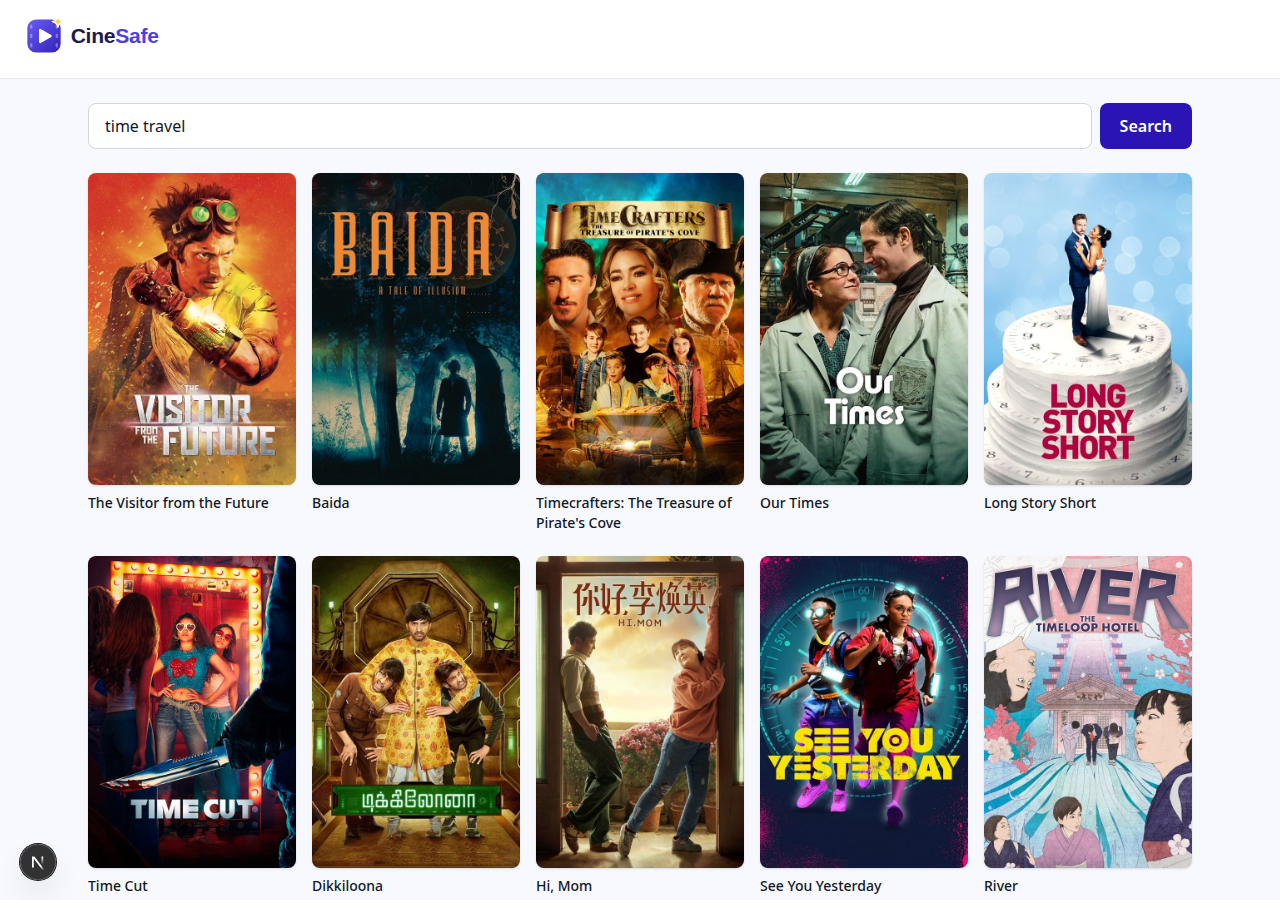
\includegraphics[width=0.75\linewidth,height=0.5279\linewidth]{./6597c1e9d916e4813a8edf0352dfe671b2cb9f8a.png}

\textbf{Hình D.1. Kết quả tìm ``time travel'', mô hình lần 1}
\end{figure}

\Needspace{20\baselineskip}
Trang chi tiết phim: poster, năm, thể loại, điểm IMDb, tóm tắt.

\begin{figure}[H]
\centering
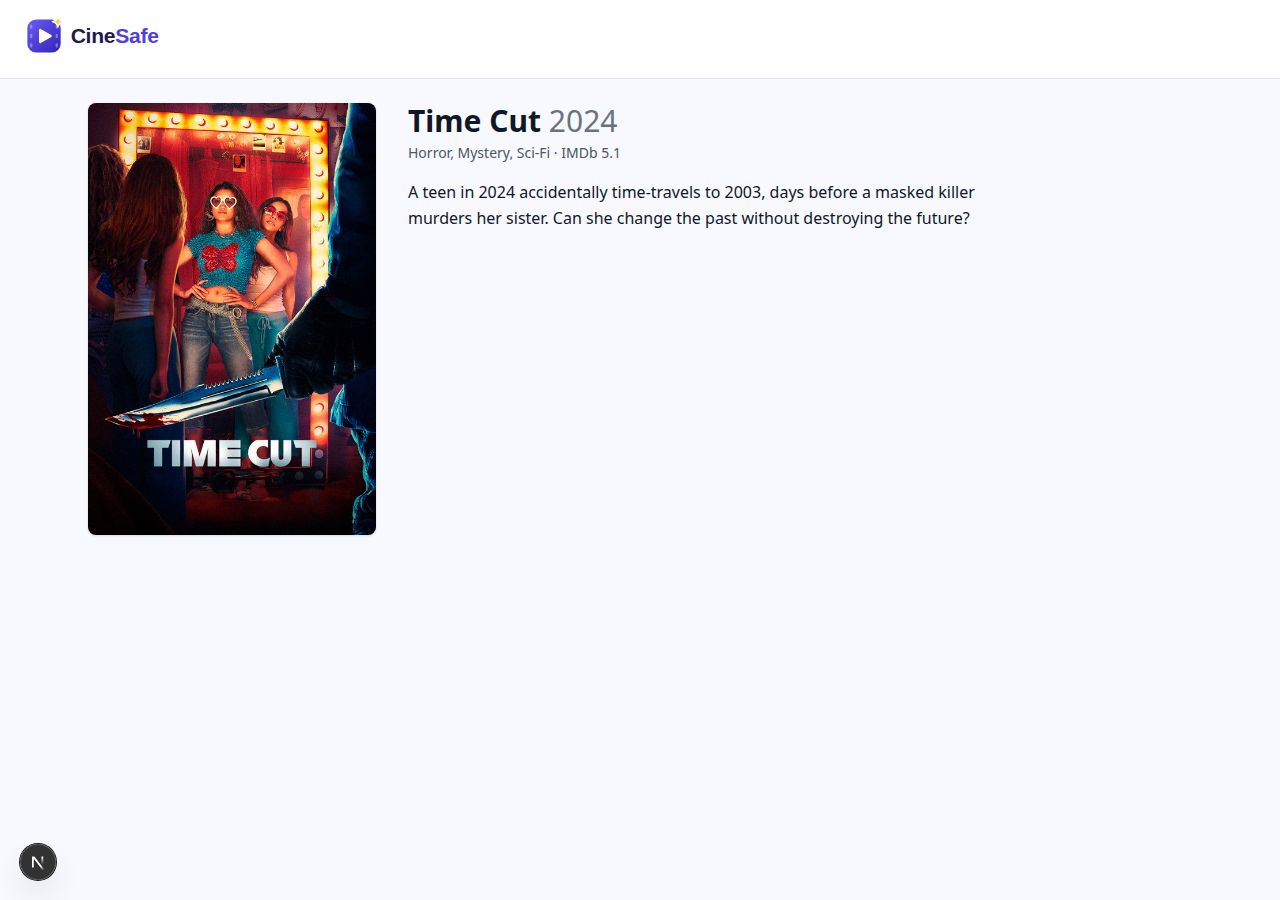
\includegraphics[width=0.75\linewidth,height=0.5279\linewidth]{./903fbcb95e5642b33f8c2d6977b8fc6860514ede.png}

\textbf{Hình D.2. Trang chi tiết phim}
\end{figure}

\Needspace{20\baselineskip}
Tìm ``the godfather'' với mô hình lần 2 (Phần III.2.5). \emph{The Godfather} (1972) đứng đầu, tiếp theo là hai phần sau. Mô hình lần 1 xếp \emph{The Godfather Part II} đầu tiên.

\begin{figure}[H]
\centering
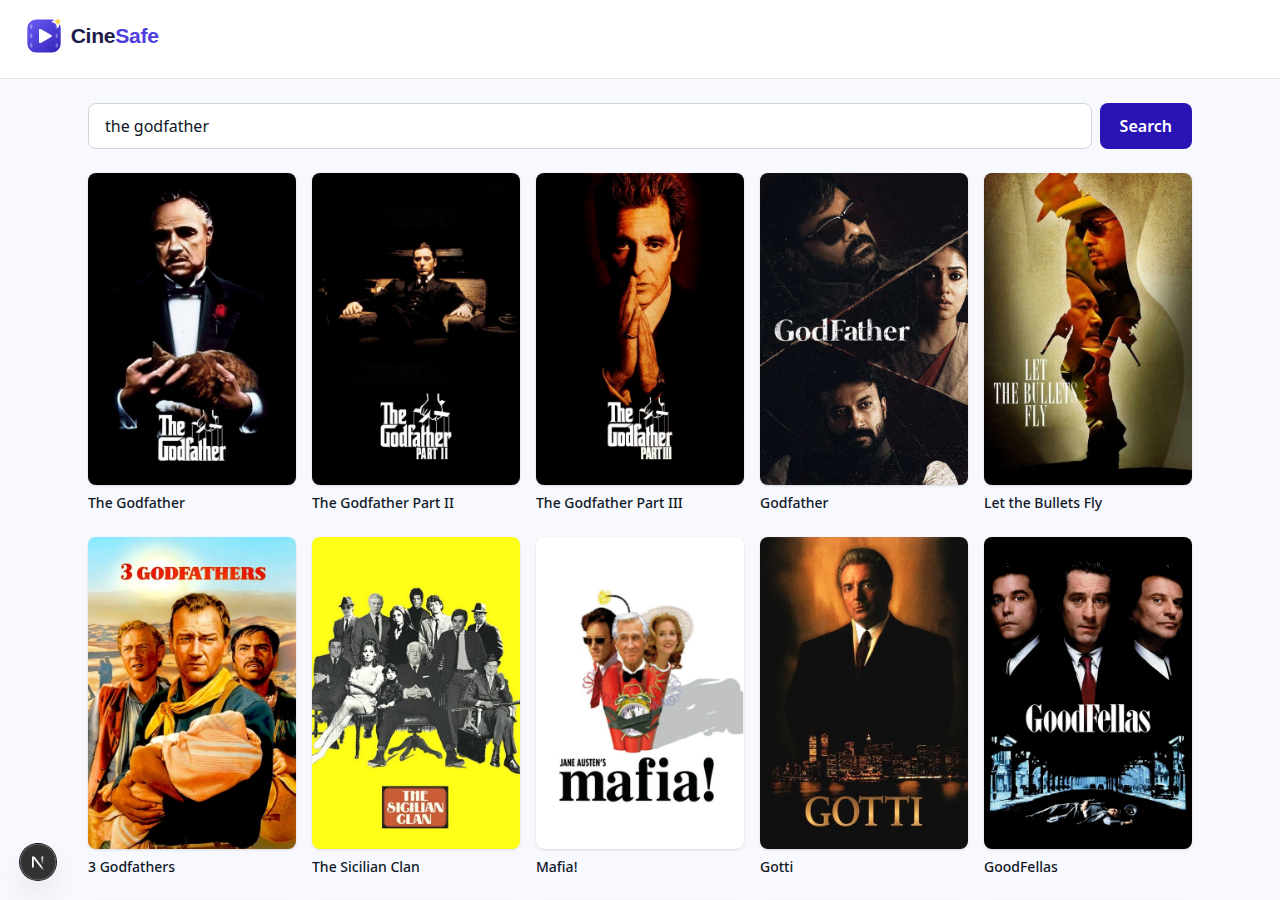
\includegraphics[width=0.75\linewidth,height=0.5279\linewidth]{./340479e21f56c6da9b908cf2b24781376f92fa32.png}

\textbf{Hình D.3. Kết quả tìm ``the godfather'', mô hình lần 2}
\end{figure}

\end{document}
